\documentclass[12pt,oneside,a4paper,PisaPhdThesis]{library//PhdThesis}
\usepackage[italian]{babel}
\usepackage[utf8]{inputenc}
\usepackage{amsmath,amssymb,amsfonts,amsthm,graphicx,mathrsfs,braket,float}
\usepackage[hidelinks]{hyperref}
\usepackage{bytefield}
\usepackage{multirow}
\usepackage{url}
\usepackage{afterpage}
\usepackage{textcomp}
\newcommand\blankpage{%
    \null
    \thispagestyle{empty}%
    \addtocounter{page}{-1}%
    \newpage
}
\setcounter{secnumdepth}{4} 
\setcounter{tocdepth}{3}
\linespread{1.0}
\graphicspath{ {./images/} }

\newlength{\defbaselineskip}
\setlength{\defbaselineskip}{\baselineskip}
\newcommand{\setlinespacing}[1]%
           {\setlength{\baselineskip}{#1 \defbaselineskip}}
\newcommand{\doublespacing}{\setlength{\baselineskip} {2.0 \defbaselineskip}}
\newcommand{\singlespacing}{\setlength{\baselineskip}{\defbaselineskip}}
\newcommand{\mycenterline}[1]{\vspace{.1cm}\newline\vspace{.1cm}\centerline{#1}}


\begin{document}
\selectlanguage{italian}

% [START] Frontespizio
\pagenumbering{gobble}

\begin{figure}
 \centering
 \vspace*{-4cm}  
\includegraphics[scale=0.7]{logo_unict.png}
 \label{fig:logoUnict}
\end{figure}


\centerline{{\LARGE UNIVERSIT\`{A} DEGLI STUDI DI CATANIA}}
\centerline{DIPARTIMENTO DI MATEMATICA E INFORMATICA}
\centerline{CORSO DI LAUREA IN INFORMATICA MAGISTRALE}
\centerline{\rule{18cm}{0.2mm}}

\vspace*{2cm}

\centerline{\LARGE{\bf RELAZIONE FINALE}}
\centerline{\LARGE{}} %salta una riga
%\centerline{\LARGE{\it SOTTOTITOLO TESI}}

\vspace*{2cm}

%\vspace*{cm}
\centerline{\rule{4cm}{0.2mm}}
\medskip
\centerline{MACHINE LEARNING}
\centerline{\rule{4cm}{0.2mm}}

\vspace*{4.0cm}
\begin{minipage}[t]{0.47\textwidth}
\raggedright{
\makebox[3cm][l]{\bf STUDENTI}\par
\makebox[3cm][l]{\it Giuseppe Giliberto W82000115}\par
\makebox[3cm][l]{\it Giuseppe Puglisi W82000112}\par
\makebox[3cm][l]{\it Giuseppe Sgroi W82000131}\par}
\end{minipage}
\vspace*{1.5cm}
\begin{minipage}[t]{0.47\textwidth}
\raggedleft{


\makebox[1.5cm][l]{\bf DOCENTE}\par
\makebox[3.6cm][l]
{\it Prof. Giovanni M. Farinella}\par \vspace*{0.5cm}
} \vspace*{0.5cm}
\end{minipage}

\centerline{\rule{18cm}{0.2mm}} 
\centerline{ANNO ACCADEMICO 2017/2018}
\newpage
\thispagestyle{empty}

% [END]

\chaptertitlestyle{serifbig}
\pagestyle{serif}

%\maketitle

\begin{frontmatter}
\setlinespacing{1.5}
\pagenumbering{roman}
\tableofcontents
\pagenumbering{arabic} \setcounter{page}{1}
\end{frontmatter}

%=====================

% [START] Capitolo 1
\chapter{Introduzione}
Il challenge di Machine Learning consiste nell’affrontare un problema di localizzazione basato su immagini, ovvero costruire un algoritmo che, data un’immagine acquisita in uno spazio noto, permetta di inferire la posizione dalla quale l’immagine è stata scattata.
\begin{figure}[H]
	\centering
	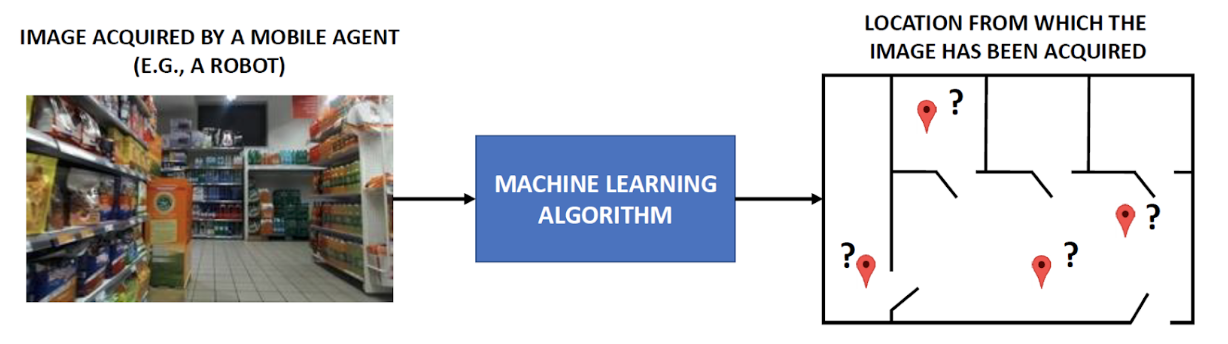
\includegraphics[scale=0.75]{image1.png}
\end{figure}
Esso può essere trattato come un problema di machine learning, e affrontato fondamentalmente in due modi:
\begin{itemize}
	\item[•]\bf Localizzazione basata su classificazione
	\item[•]\bf Localizzazione basata su regressione
\end{itemize}	
\begin{figure}[H]
	\centering
	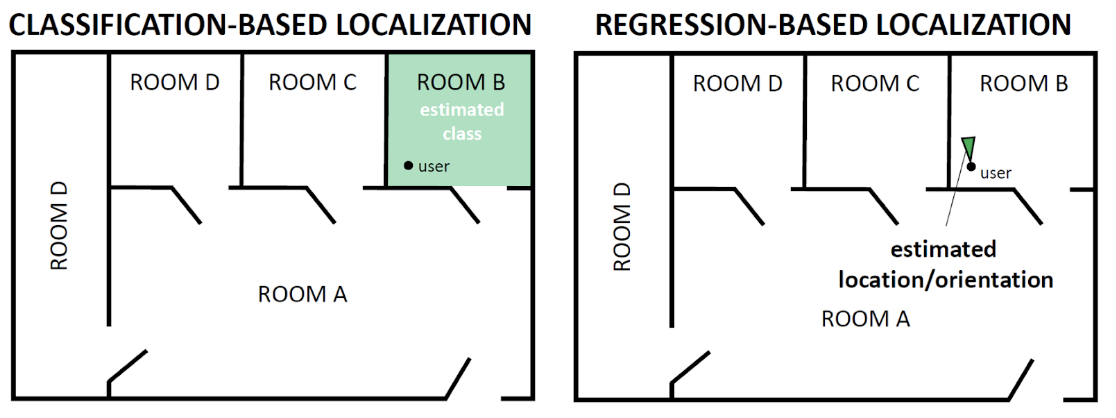
\includegraphics[scale=0.75]{image2.png}
\end{figure}
La sorgente dei dati in esame è una camera incorporata in un robot che effettua un determinato cammino in un supermercato. Il robot acquisisce un video che successivamente viene suddiviso nei suoi frames. Essi faranno parte del dataset.
\\
Il {\bf problema di classificazione} consiste nella localizzazione del robot in uno dei 16 reparti del supermercato.
\\
Il {\bf problema di regressione}, invece, consiste nel prevedere la posizione del robot nei momenti dell’acquisizione del video.
\newline
Il dataset quindi è formato dalle immagini e da un insieme di relative etichette che rappresentano rispettivamente:
\begin{itemize}
	\item[•] Posizione rispetto all’asse X
	\item[•] Posizione rispetto all’asse Y
	\item[•] Orientamente etichettato da U e V
	\item[•] Classe di appartenenza
\end{itemize}	
Per risolvere i problemi di classificazione e regressione abbiamo implementato e confrontato i seguenti algoritmi: {\bf MLP}, {\bf MLP Deep}, {\bf VGG16 pre-addestrata} con opportuno fine tuning. \\
Per l’esecuzione dei test è stata utilizzata la seguente configurazione hardware/software:
\begin{itemize}
	\item[-] {\bf O.S}: Ubuntu 18.04
	\item[-] {\bf CUDA}: v9.1.85
	\item[-] {\bf PyTorch}: v0.4
	\item[-] {\bf CPU}: Intel core i7 di 2° generazione
	\item[-] {\bf RAM}: 8 GB ddr3
	\item[-] {\bf GPU}: Nvidia geForce GTX 1080ti
\end{itemize}	

% [END]

%=====================

% [START] Capitolo 
\chapter{Esperimenti}

I primi esperimenti effettuati vertono sulla risoluzione del {\bf problema di classificazione}.
\newline
Abbiamo implementato le seguenti architetture di rete:
\begin{itemize}
	\item[•]{\bf MLP}: semplice MLP con un livello nascosto
	\item[•]{\bf MLP Deep}: MLP con due livelli nascosti
	\item[•]{\bf VGG16 pre-addestrata}: viene ripresa l’architettura di rete VGG16 e inizializzata con i pesi della stessa rete pre-addestrata su un task differente. Vengono poi effettuate diverse strategie di fine-tuning della rete
\end{itemize}	
Per la risoluzione del {\bf problema di regressione} abbiamo effettuato gli esperimenti essenzialmente con le medesime architetture, andando però a modellare le architetture per la semantica del task.
\\
\\
Per le reti MLP viene effettuata la normalizzazione delle immagini per media e deviazione standard del training set, mentre per quanto riguarda la rete VGG16 pre-addestrata viene effettuata la normalizzazione delle immagini per media e deviazione standard del dataset “ImageNet” su cui è stata allenata la rete VGG16.

\section{Architettura MLP}

\subsection{Classificazione}
Utilizziamo una semplice architettura MLP con tre livelli:
\begin{itemize}
	\item[•]Livello di input: 110592 neuroni. In input abbiamo immagini di dimensione 144x256x3
	\item[•]Livello nascosto: 512 neuroni
	\item[•]Livello di output: 16 neuroni (Softmax)
\end{itemize}
\begin{figure}[H]
	\centering
	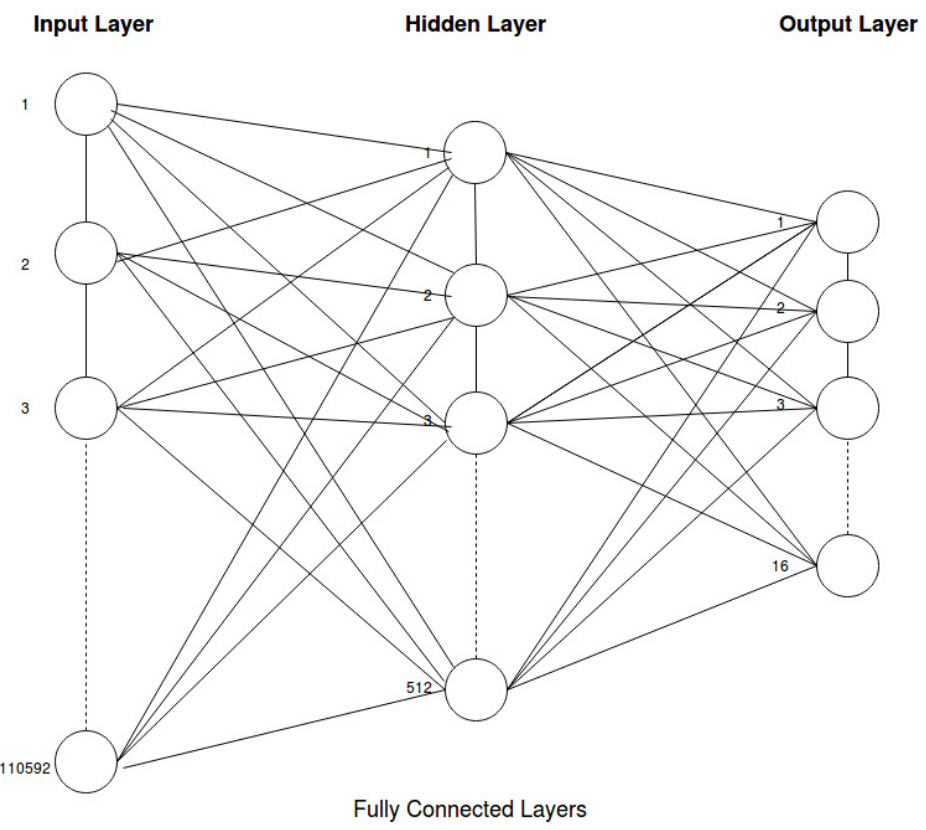
\includegraphics[scale=0.6]{image3.png}
\end{figure}
Per la procedura di training utilizziamo: 
\begin{itemize}
	\item[•]Learning rate: 0.00001
	\item[•]Momentum: 0.9
	\item[•]Weight decay: 0.000001
\end{itemize}
Come loss function utilizziamo cross entropy loss, come funzione di attivazione utilizziamo ReLU, mentre come metodo di learning utilizziamo SGD.
\newline
Abbiamo allenato il modello per 150 epoche, ed abbiamo ottenuto i seguenti risultati:

\subsubsection{Accuracy}
\begin{figure}[H]
	\centering
	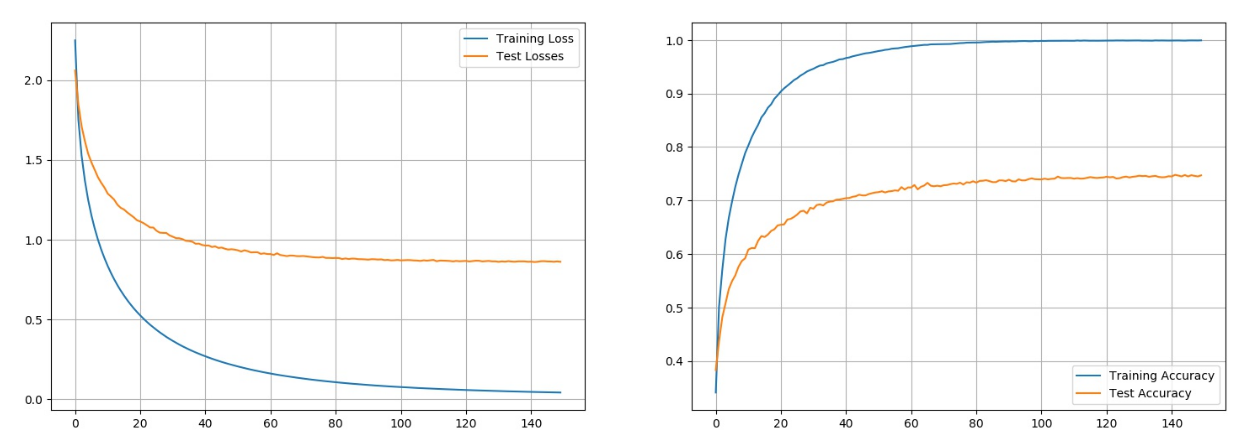
\includegraphics[scale=0.65]{image4.png}
\end{figure}
Dai due plot si osserva come sul validation la loss rimane relativamente alta, e l’accuracy relativamente bassa. Da ciò si intuisce che questo approccio non dà i risultati sperati.

\subsubsection{Matrice di confusione}
\begin{figure}[H]
	\centering
	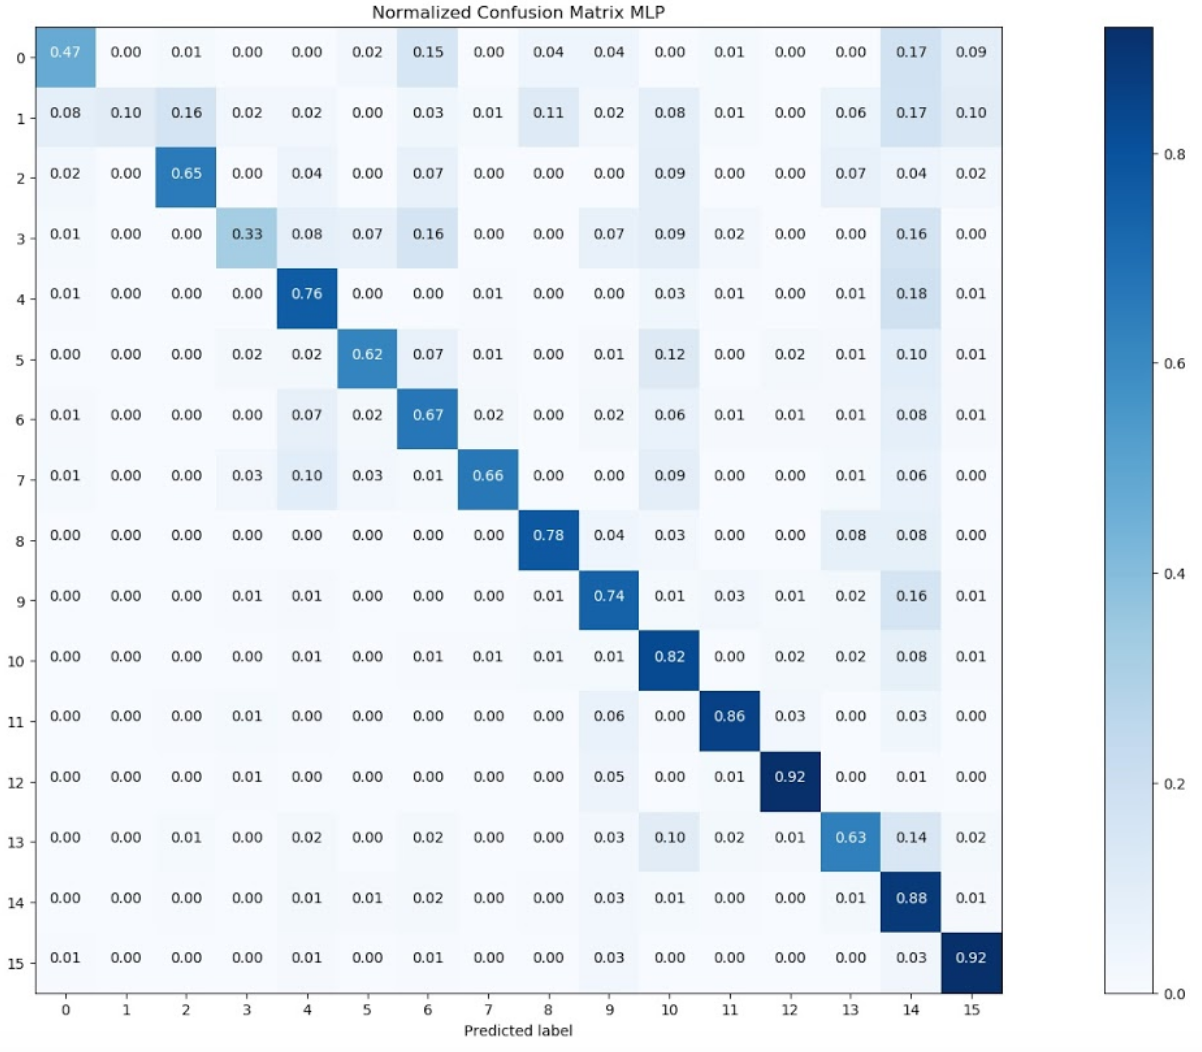
\includegraphics[scale=0.5]{image5.png}
\end{figure}
Nella matrice di confusione, l'elemento di indici i,j indica quanti elementi {\bf appartenenti alla classe i sono stati classificati come appartenenti alla classe j}. \\
In pratica un buon classificatore presenterebbe una matrice di confusione con i numeri sulla diagonale principale alti e i numeri fuori dalla diagonale principale bassi. \\
Attraverso essa è possibile confrontare visivamente i valori reali con quelli stimati dal modello e quindi controllare quali elementi vengono classificati correttamente e quali no. Gli score F1 ne sono una conferma.

\subsubsection{Score F1 e Score mF1}
\begin{center}
\begin{tabular}{| l | l | l | l |}
	\hline
	Classe & Score F1 \\ \hline
	0 & 0.57 \\ \hline
	1 & 0.19 \\ \hline
	2 & 0.61 \\ \hline
	3 & 0.44\\ \hline
	4 & 0.74 \\ \hline
	5 & 0.70\\ \hline
	6 & 0.58 \\ \hline
	7 & 0.75\\ \hline
	8 & 0.75 \\ \hline
	9 & 0.78\\ \hline
	10 & 0.77 \\ \hline
	11 & 0.87 \\ \hline
	12 & 0.88 \\ \hline
	13 & 0.72 \\ \hline
	14 & 0.75\\ \hline
	15 & 0.87 \\ \hline 
	{\bf Score mF1} & 0.68 \\ \hline							
\end{tabular}
\end{center}
Gli score F1 indicano le performance del classificatore MLP per ogni classe. Per ottenere un indicatore generale di performance viene calcolata la media dei punteggi relativi alle singole classi, che è relativamente basso e pari a 0.68
\newline
Con questa architettura otteniamo una {\bf accuracy} di {\bf 0.75} sul validation. 

\subsection{Regressione}
Utilizziamo la semplice architettura MLP con tre livelli vista sopra, con la sola differenza che il livello di output avrà 4 neuroni e non più il classificatore softmax:
\begin{itemize}
	\item[•]Livello di input: 110592 neuroni. In input abbiamo immagini di dimensione 144x256x3
	\item[•]Livello nascosto: 512 neuroni
	\item[•]Livello di output: 4 neuroni
\end{itemize}
\begin{figure}[H]
	\centering
	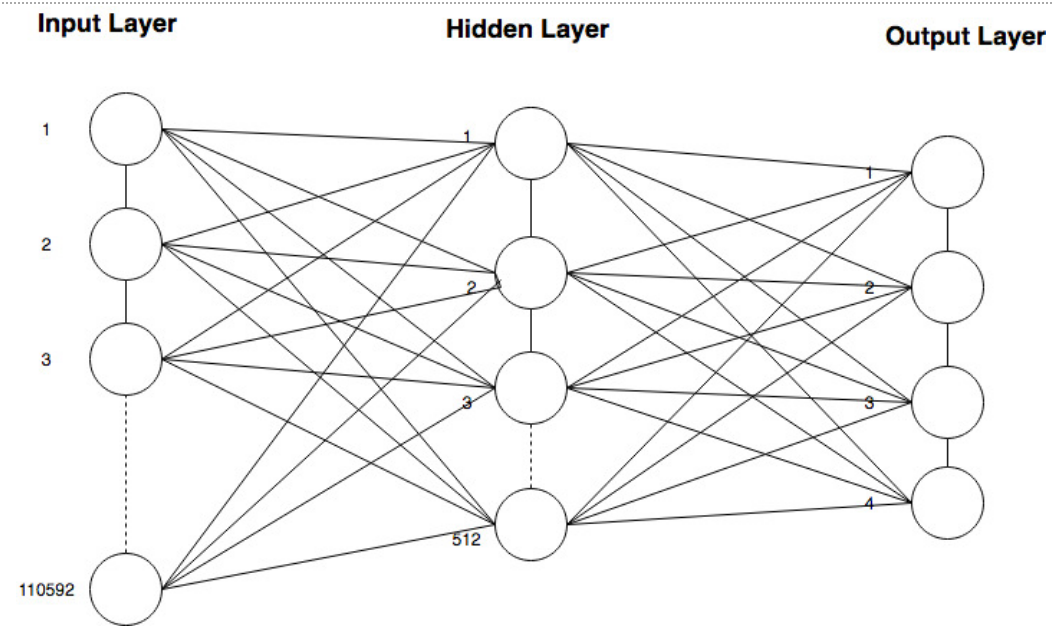
\includegraphics[scale=0.6]{image6.png}
\end{figure}
A differenza di quanto fatto per la classificazione, l’ultimo livello non sarà più softmax, in quanto non abbiamo più bisogno di una distribuzione di probabilità sulle classi, ma un vettore di 4 parametri corrispondenti ai valori x, y, u, v che localizzano un’immagine.
Per la procedura di training utilizziamo: 
\begin{itemize}
	\item[•]Learning rate: 0.00001
	\item[•]Momentum: 0.9
	\item[•]Weight decay: 0.000001
\end{itemize}
Come loss function da ottimizzare utilizziamo MSE loss, come funzione di attivazione utilizziamo Tanh, mentre come metodo di learning utilizziamo SGD.
\newline
Poiché abbiamo da stimare quattro numeri reali x, y, u, v, utilizziamo a tale scopo quattro loss functions, una per ogni valore, le quali verranno ottimizzate assieme durante la procedura di training.
\newline
Abbiamo allenato il modello per 150 epoche, ed abbiamo ottenuto i seguenti risultati:

\subsubsection{Loss functions}
\begin{figure}[H]
	\centering
	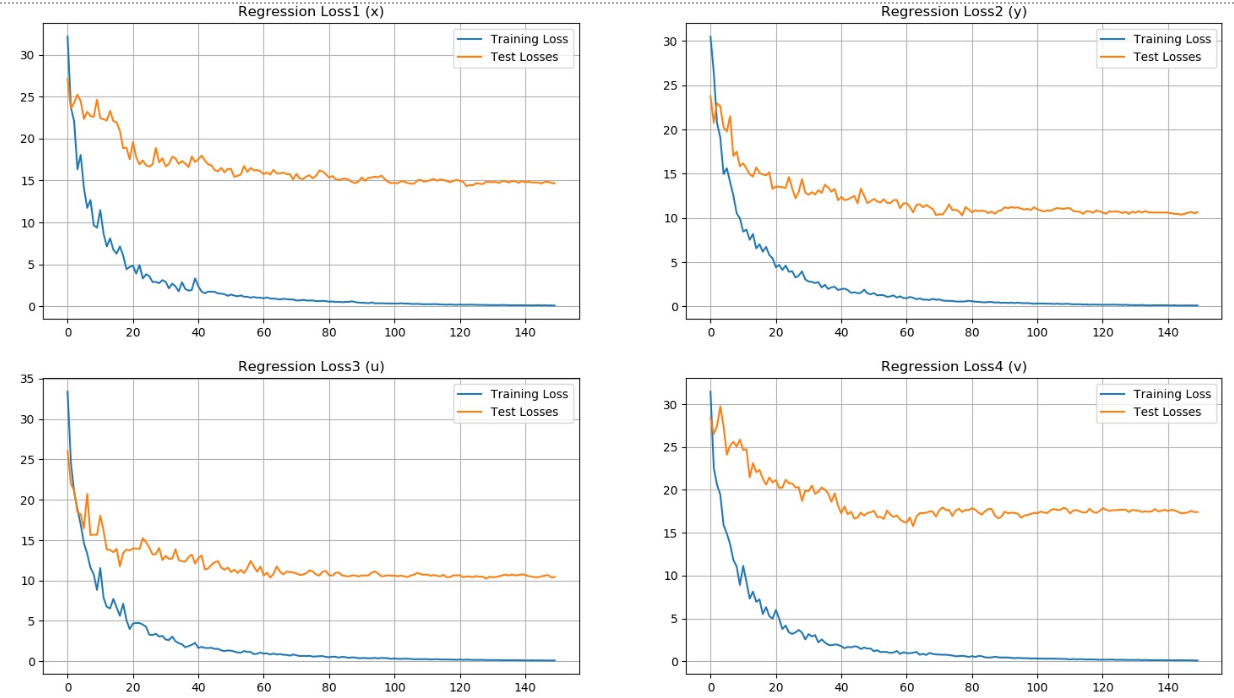
\includegraphics[scale=0.70]{image7.png}
\end{figure}
Come è possibile osservare dai 4 plot le loss di validation non raggiungono un valore ottimale, come, invece, accade sul training.

\subsubsection{MSE errors}
\begin{center}
	\begin{tabular}{| l | l | l | l |}
		\hline
		MSE sul parametro X & 45.84 \\ \hline
		MSE sul parametro Y & 8.10 \\ \hline
		MSE sul parametro U & 0.34 \\ \hline
		MSE sul parametro V & 0.33 \\ \hline							
	\end{tabular}
\end{center}

\subsubsection{REC curves}
Le REC curve rappresentano un metodo grafico per valutare la bontà di un metodo di regressione. Inoltre, alla curva è spesso associata l'area sopra la curva (AOC) per offrire una misura dell'errore del metodo.
\begin{figure}[H]
	\centering
	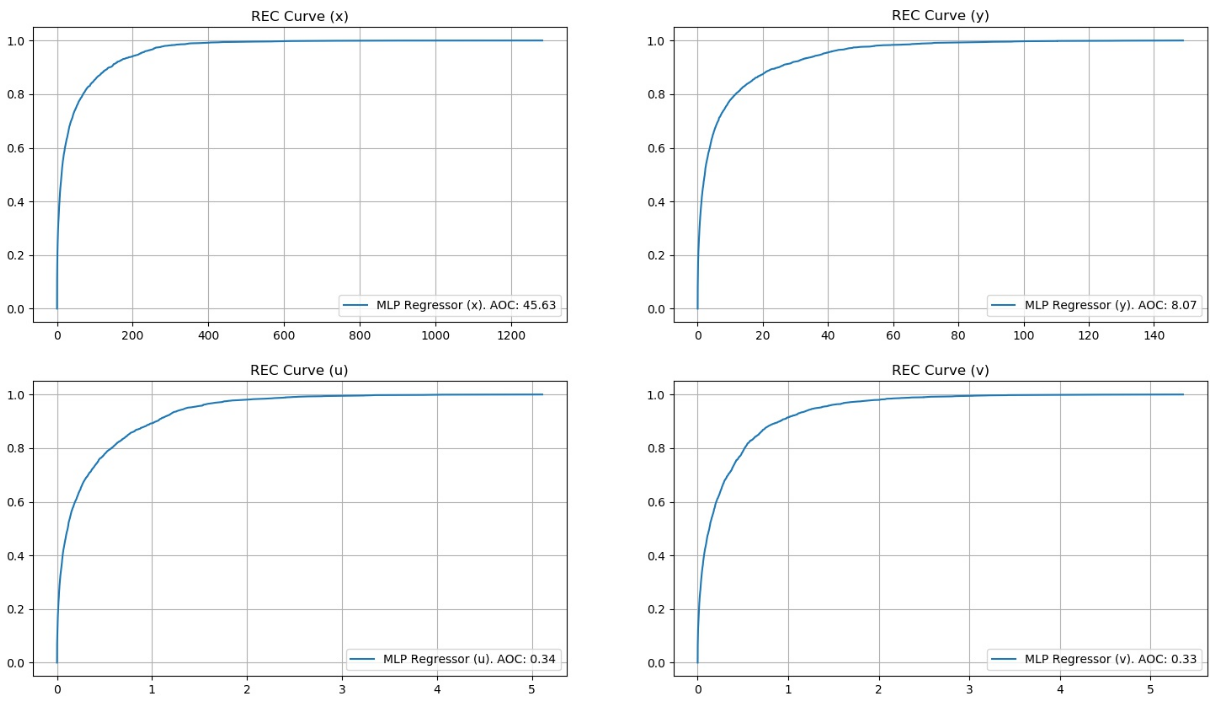
\includegraphics[scale=0.70]{image8.png}
\end{figure}

\subsubsection{RMS error}
errore RMS (Root Mean Square) medio e mediano relativo a posizione (in metri) e orientamento (in gradi):
\begin{center}
	\begin{tabular}{| l | l | l | l |}
		\hline
		Mean location error & 5.7011 \\ \hline
		Median location error & 4.3916 \\ \hline
		Mean orientation error & 46.4265 \\ \hline
		Median orientation error & 29.7348 \\ \hline							
	\end{tabular}
\end{center}

%==========================================
\newpage

\section{Architettura MLP Deep}

\subsection{Classificazione}
Utilizziamo un’architettura di rete molto simile a quella appena vista, con la differenza dell’aggiunta di un secondo livello nascosto:
\begin{itemize}
	\item[•]Livello di input: 110592 neuroni. In input abbiamo immagini di dimensione 144x256x3
	\item[•]2 livelli nascosti: 512 neuroni ciascuno
	\item[•]Livello di output: 16 neuroni (Softmax)
\end{itemize}
\begin{figure}[H]
	\centering
	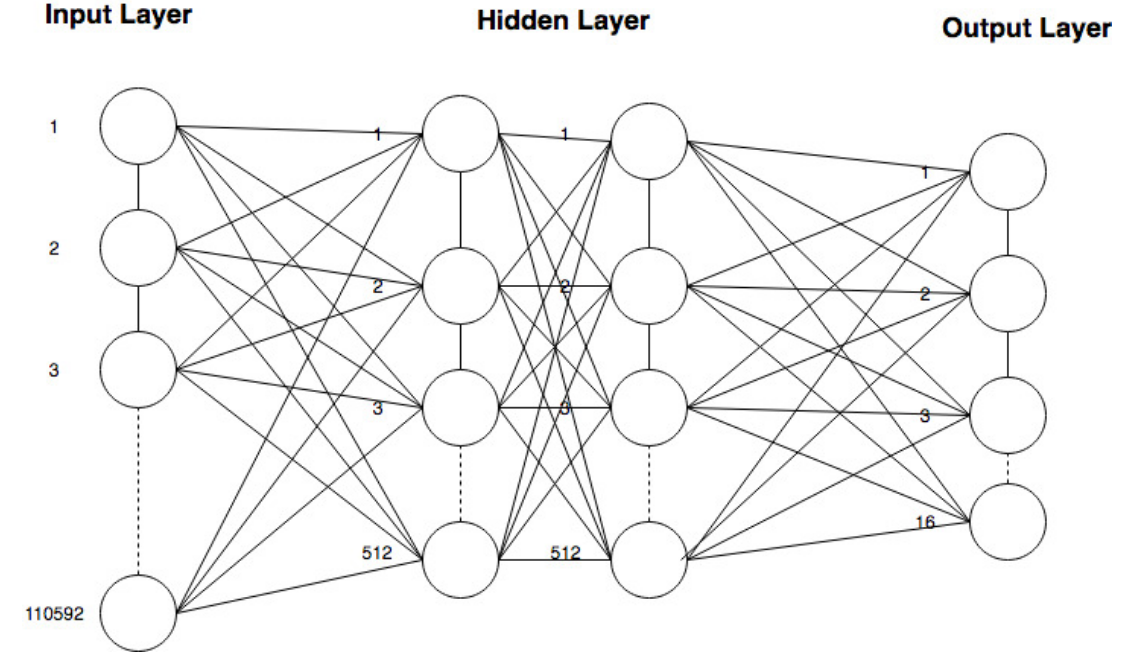
\includegraphics[scale=0.6]{image9.png}
\end{figure}
Per la procedura di training utilizziamo: 
\begin{itemize}
	\item[•]Learning rate: 0.00001
	\item[•]Momentum: 0.9
	\item[•]Weight decay: 0.000001
\end{itemize}
Come loss function utilizziamo cross entropy loss, come funzione di attivazione utilizziamo ReLU, mentre come metodo di learning utilizziamo SGD.
\newline
Abbiamo allenato il modello per 150 epoche, ed abbiamo ottenuto i seguenti risultati:
\subsubsection{Accuracy}
\begin{figure}[H]
	\centering
	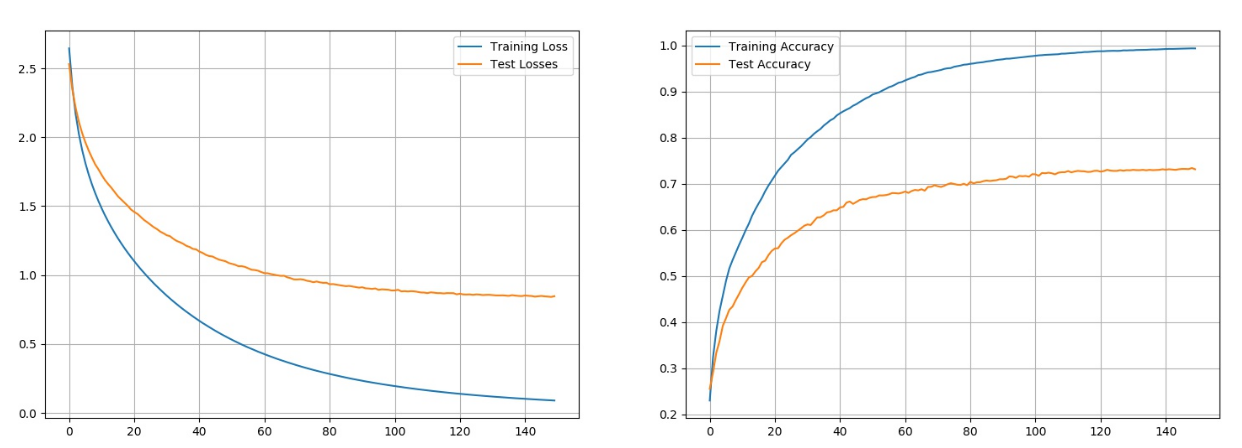
\includegraphics[scale=0.65]{image10.png}
\end{figure}
Anche in questo caso, dai due plot, si osserva come sul validation la loss rimane relativamente alta, e l’accuracy relativamente bassa. Da ciò si intuisce che anche questo approccio non dà i risultati sperati.

\subsubsection{Matrice di confusione}
\begin{figure}[H]
	\centering
	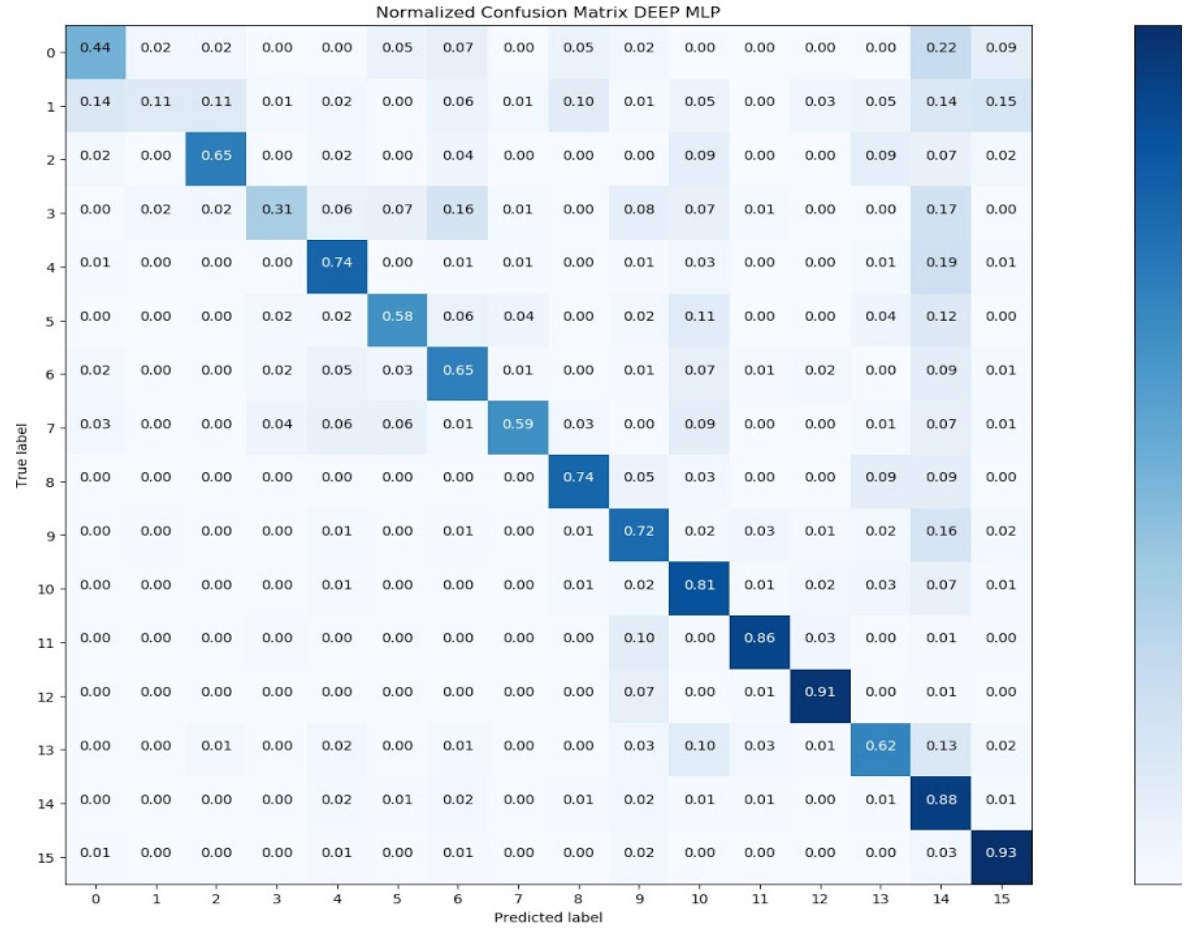
\includegraphics[scale=0.5]{image11.png}
\end{figure}
Dalla matrice di confusione possiamo vedere sulla diagonale principale i rates  in percentuale che sussistono tra le etichette predette e quelle reali. \\
A conferma di questi valori si possono osservare gli score F1.


\subsubsection{Score F1 e Score mF1}
\begin{center}
	\begin{tabular}{| l | l | l | l |}
		\hline
		Classe & Score F1 \\ \hline
		0 & 0.52 \\ \hline
		1 & 0.19 \\ \hline
		2 & 0.61 \\ \hline
		3 & 0.43\\ \hline
		4 & 0.74 \\ \hline
		5 & 0.65\\ \hline
		6 & 0.57 \\ \hline
		7 & 0.68\\ \hline
		8 & 0.71 \\ \hline
		9 & 0.75\\ \hline
		10 & 0.76 \\ \hline
		11 & 0.86 \\ \hline
		12 & 0.87 \\ \hline
		13 & 0.71 \\ \hline
		14 & 0.74\\ \hline
		15 & 0.85 \\ \hline 
		{\bf Score mF1} & 0.67 \\ \hline							
	\end{tabular}
\end{center}
Come è possibile vedere, anche in questo caso, otteniamo un score mF1 relativamente basso e pari a 0.67.
\newline
Con questa architettura otteniamo una {\bf accuracy} di {\bf 0.73} sul validation. 

\subsection{Regressione}
L’architettura di rete è la seguente:
\begin{itemize}
	\item[•]Livello di input: 110592 neuroni. In input abbiamo immagini di dimensione 144x256x3
	\item[•]2 livelli nascosti: 512 neuroni ciascuno
	\item[•]Livello di output: 4 neuroni
\end{itemize}
\begin{figure}[H]
	\centering
	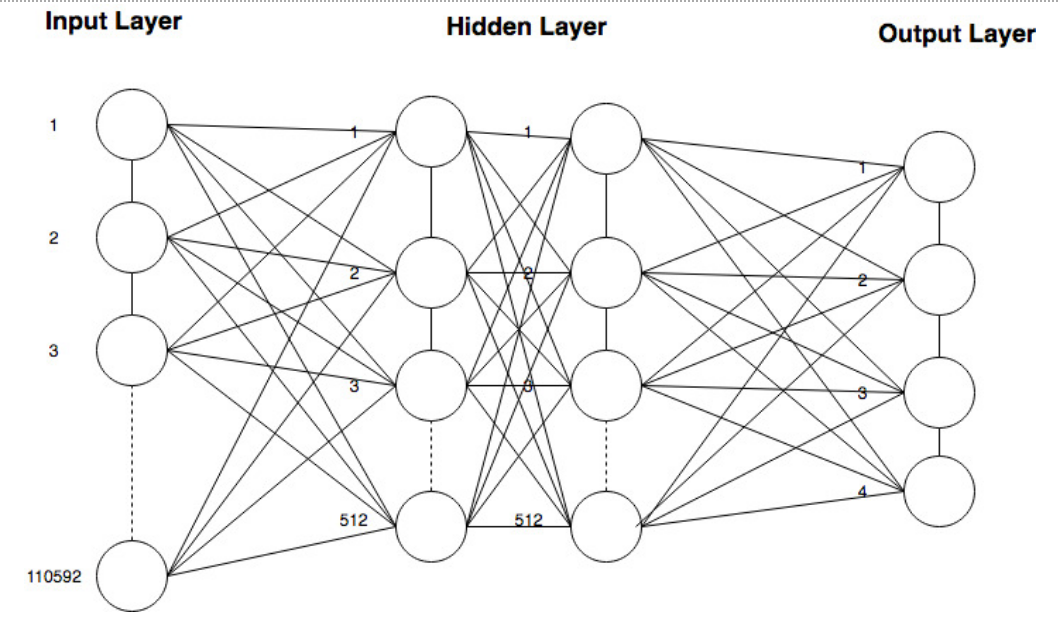
\includegraphics[scale=0.6]{image12.png}
\end{figure}
Essendo un problema di regressione, il livello di output sarà costituito da 4 neuroni corrispondenti ai valori x, y, u, v che localizzano un’immagine.
Per la procedura di training utilizziamo: 
\begin{itemize}
	\item[•]Learning rate: 0.00001
	\item[•]Momentum: 0.9
	\item[•]Weight decay: 0.000001
\end{itemize}
Come loss function da ottimizzare utilizziamo MSE loss, come funzione di attivazione utilizziamo Tanh, mentre come metodo di learning utilizziamo SGD.
Poiché abbiamo da stimare quattro numeri reali x, y, u, v, utilizziamo a tale scopo quattro loss functions, una per ogni valore, le quali verranno ottimizzate assieme durante la procedura di training.
Abbiamo allenato il modello per 150 epoche, ed abbiamo ottenuto i seguenti risultati:

\subsubsection{Loss functions}
\begin{figure}[H]
	\centering
	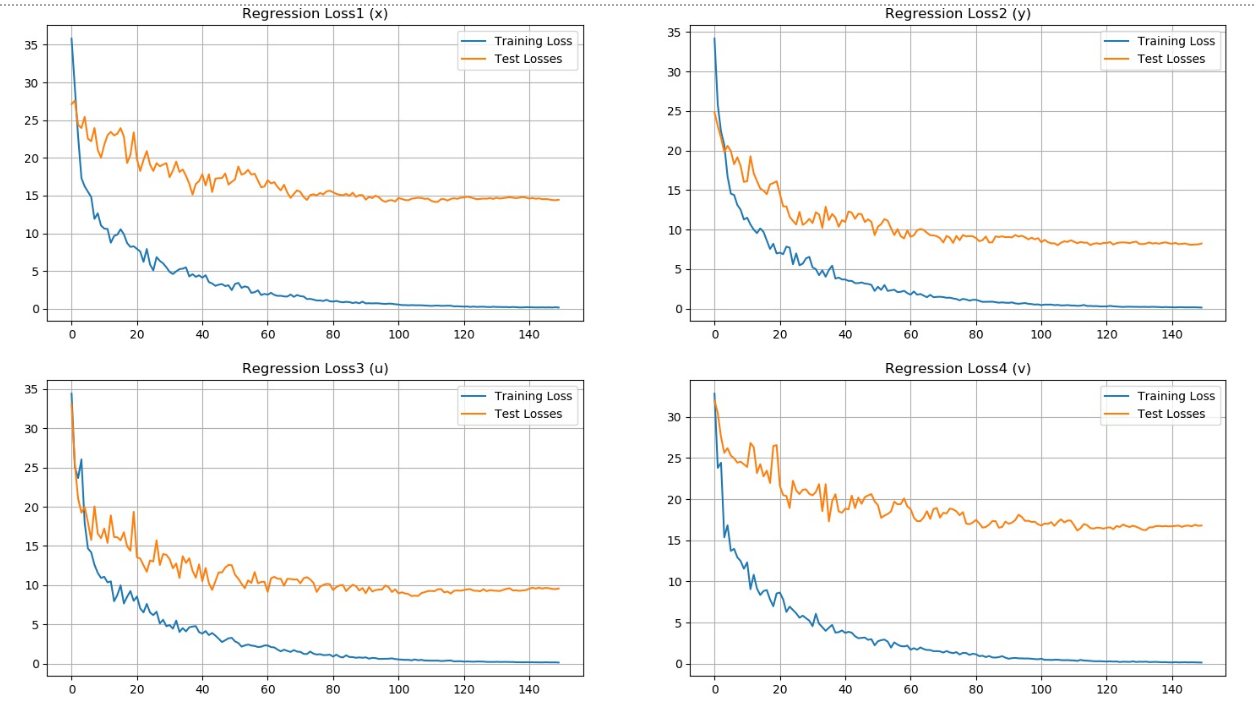
\includegraphics[scale=0.70]{image13.png}
\end{figure}
Anche in questo caso i plot mostrano dei risultati relativamente alti per le loss functions sul validation. 

\subsubsection{MSE errors}
\begin{center}
	\begin{tabular}{| l | l | l | l |}
		\hline
		MSE sul parametro X & 44.92 \\ \hline
		MSE sul parametro Y & 8.19 \\ \hline
		MSE sul parametro U & 0.33 \\ \hline
		MSE sul parametro V & 0.34 \\ \hline							
	\end{tabular}
\end{center}

\subsubsection{REC curves}
\begin{figure}[H]
	\centering
	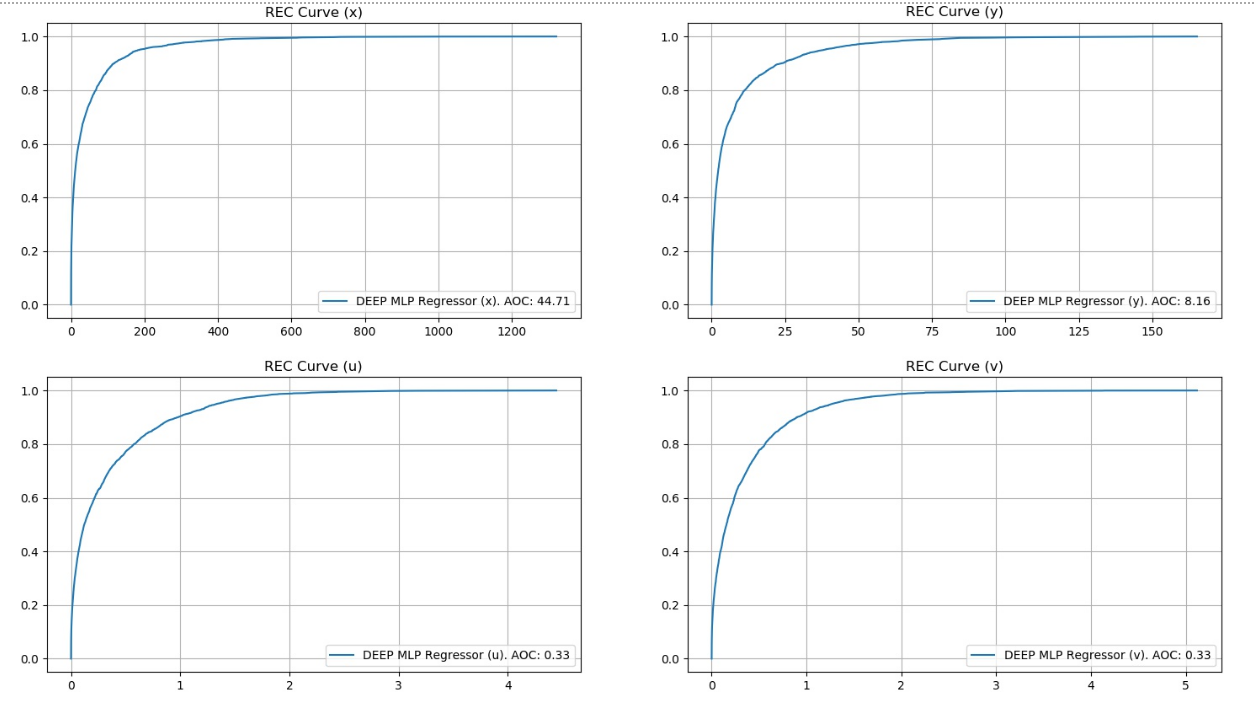
\includegraphics[scale=0.70]{image14.png}
\end{figure}

\subsubsection{RMS error}
errore RMS (Root Mean Square) medio e mediano relativo a posizione (in metri) e orientamento (in gradi):
\begin{center}
	\begin{tabular}{| l | l | l | l |}
		\hline
		Mean location error & 5.6398 \\ \hline
		Median location error & 4.4736 \\ \hline
		Mean orientation error & 48.5022 \\ \hline
		Median orientation error & 33.9735 \\ \hline							
	\end{tabular}
\end{center}

%==========================================

\newpage
\section{Architettura VGG16 pre-addestrata}
Come si è osservato negli esperimenti sovrastanti, i risultati raggiunti non sono stati soddisfacenti, in particolare i plot mostravano che la loss di validation non decresceva così come quella di training. Questo è un chiaro esempio di modelli che non generalizzano a dovere. \\
Risulta quindi necessario affrontare un’altra tecnica chiamata transfer learning che ci aiuta ad allenare modelli più accurati, con la speranza di ottenere risultati ottimali.
\\ \\
Abbiamo sfruttato l’architettura di rete {\bf VGG-16} pre-addestrata sul dataset “ImageNet” per affrontare i nostri task di classificazione e regressione.\\
Diamo uno sguardo all’architettura generale:
\begin{figure}[H]
	\centering
	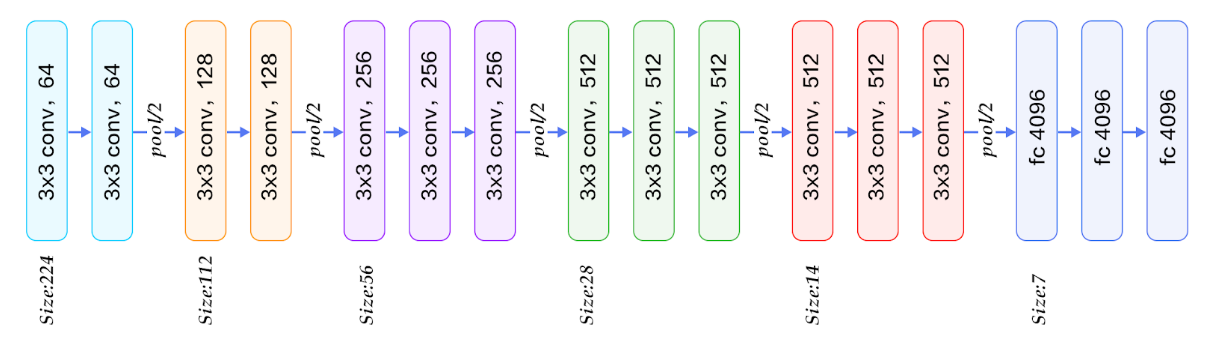
\includegraphics[scale=0.70]{image15.png}
\end{figure}
L’architettura contiene cinque blocchi convoluzionali ed un blocco fully connected finale, e tutti i parametri sono stati allenati per la classificazione su 1000 classi. \\
La rete prende in input immagini 244x244x3 sotto forma di batches, che vengono normalizzate con media e deviazione standard del dataset “ImageNet”. \\
Abbiamo quindi la necessità, come primo passo, di adattare l’architettura alla dimensione dei nostri input, in modo tale da poter accettare in input immagini 144x256x3:
\begin{figure}[H]
	\centering
	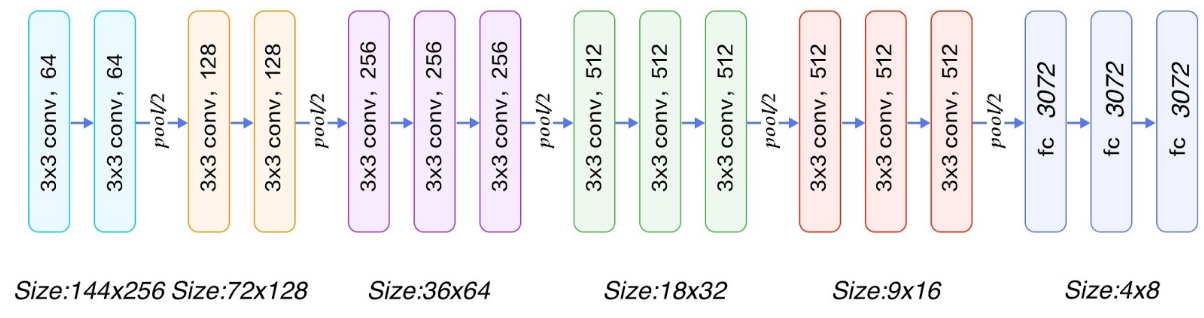
\includegraphics[scale=0.70]{image16.png}
\end{figure}
Successivamente abbiamo seguito due differenti approcci di fine-tuning sulla rete:
\begin{itemize}
	\item[1.]“Freeze” dei parametri di tutti i livelli convoluzionali, a differenza di quelli dell’ultimo blocco fully connected
	\item[2.]“Freeze” dei parametri di tutti i livelli convoluzionali, a differenza di quelli dell’ultimo blocco convoluzionale e del blocco fully connected
	\item[3.]“Freeze” dei parametri di tutti i livelli convoluzionali, a differenza di quelli degli ultimi due blocchi convoluzionali, del blocco fully connected e con l’aggiunta di data augmentation. Questo approccio rappresenterà il nostro metodo proposto
\end{itemize}

\section{VGG16 pre-addestrata: {1\textdegree} approccio}
Sono stati freezati tutti i livelli del modulo “features” che contiene i blocchi convoluzionali. In questo modo verranno aggiornati solamente i parametri dei livelli del modulo “classifier”, lasciano invariati quelli di tutti i blocchi convoluzionali.

\subsection{Classificazione}
\begin{figure}[H]
	\centering
	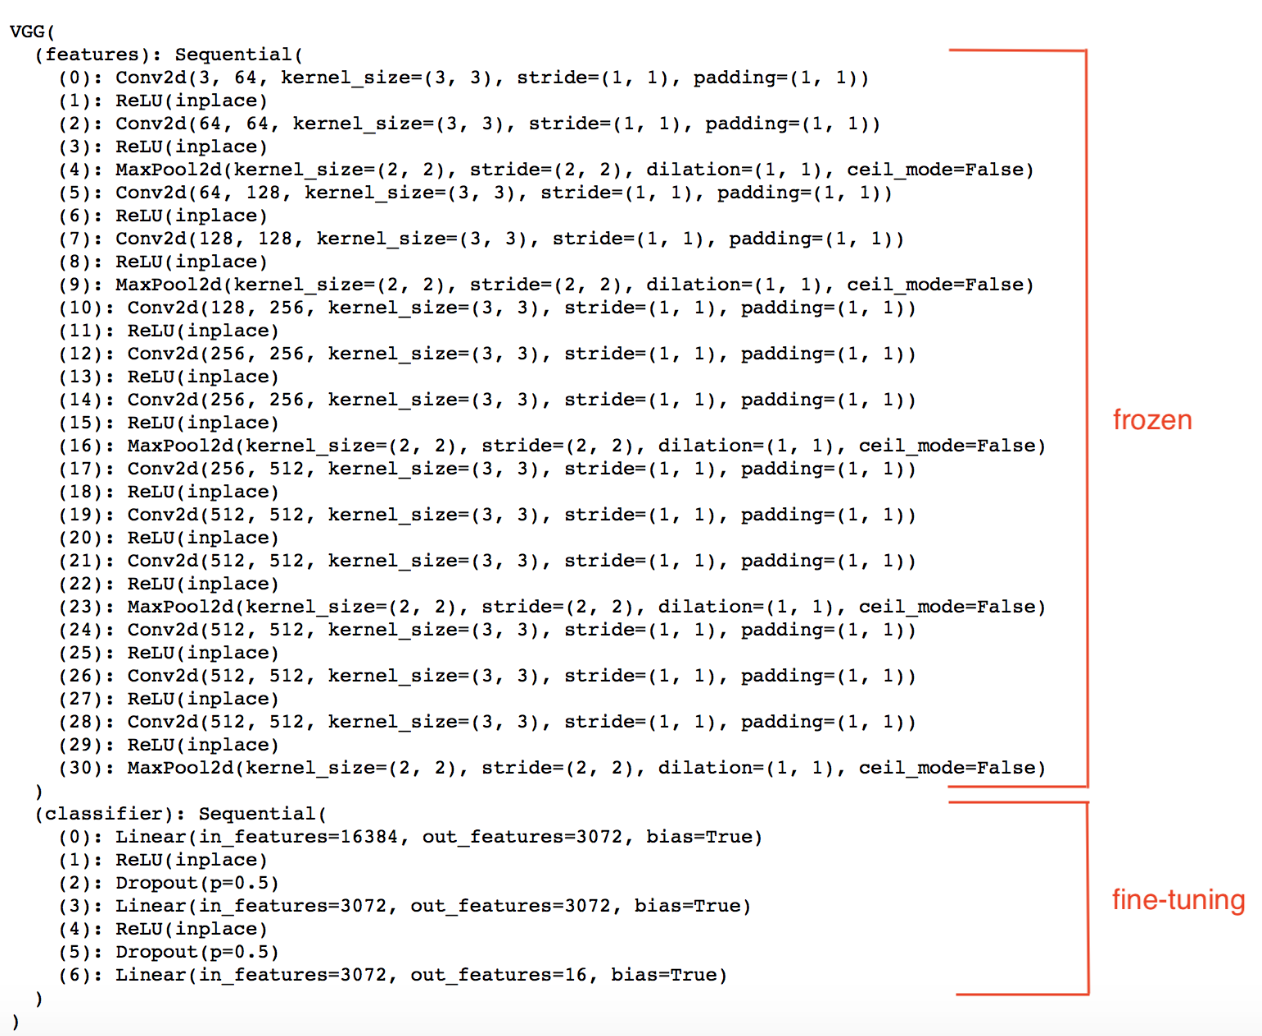
\includegraphics[scale=0.70]{image17.png}
\end{figure}
Poichè il task di classificazione richiede in output 16 classi, sono stati modificati gli ultimi livelli lineari impostando a 16 le features di output dell’ultimo livello con classificatore softmax.
Per la procedura di training utilizziamo: 
\begin{itemize}
	\item[•]Learning rate: 0.00001
	\item[•]Momentum: 0.9
	\item[•]Weight decay: 0.000001
\end{itemize}
Come loss function utilizziamo cross entropy loss, come funzione di attivazione utilizziamo ReLU, mentre come metodo di learning utilizziamo SGD. \\
Abbiamo allenato il modello per 400 epoche, ed abbiamo ottenuto i seguenti risultati:

\subsubsection{Accuracy}
\begin{figure}[H]
	\centering
	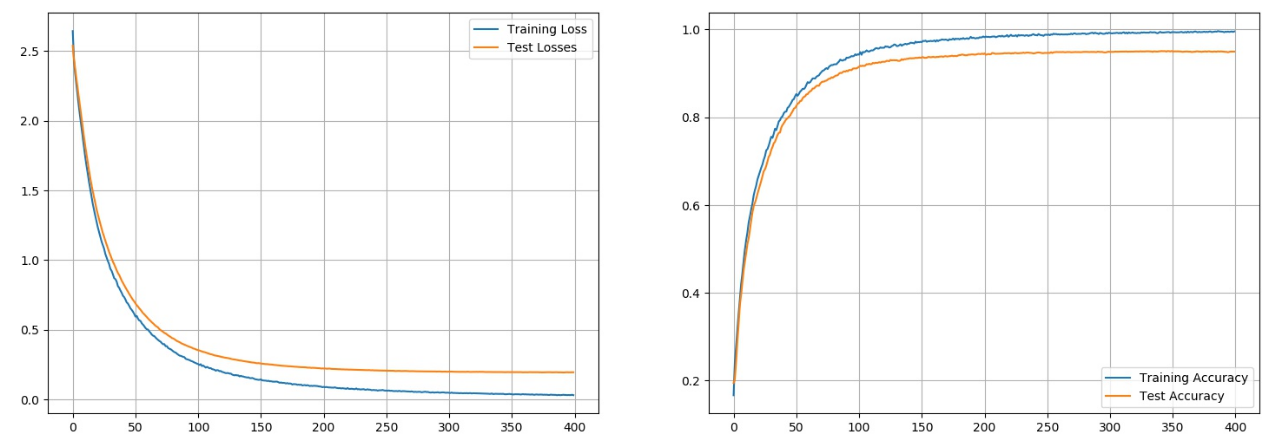
\includegraphics[scale=0.65]{image18.png}
\end{figure}
Dai plot, di cui sopra, possiamo osservare che le CNN danno risultati ampiamenti migliori. Infatti siamo riusciti ad avvicinare quanto più possibile la loss di validation a quella di training. 

\subsubsection{Matrice di confusione}
\begin{figure}[H]
	\centering
	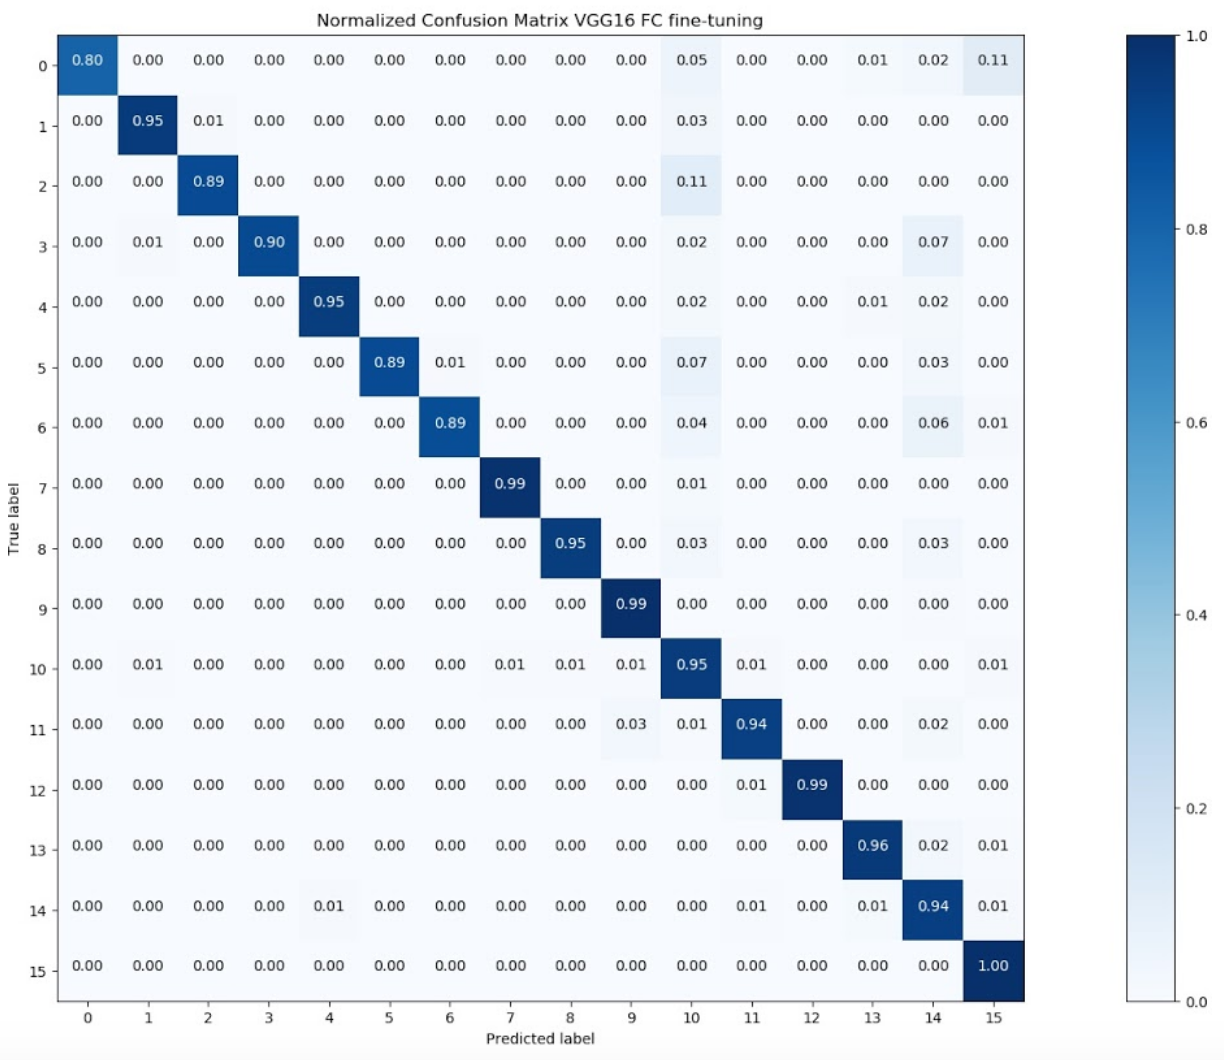
\includegraphics[scale=0.5]{image19.png}
\end{figure}
Anche dalla matrice di confusione vengono evidenziati miglioramenti avvenuti con le CNN.

\subsubsection{Score F1 e Score mF1}
\begin{center}
	\begin{tabular}{| l | l | l | l |}
		\hline
		Classe & Score F1 \\ \hline
		0 & 0.89 \\ \hline
		1 & 0.95 \\ \hline
		2 & 0.93 \\ \hline
		3 & 0.94 \\ \hline
		4 & 0.96 \\ \hline
		5 & 0.93 \\ \hline
		6 & 0.93 \\ \hline
		7 & 0.98 \\ \hline
		8 & 0.95 \\ \hline
		9 & 0.99 \\ \hline
		10 & 0.92 \\ \hline
		11 & 0.95 \\ \hline
		12 & 0.99 \\ \hline
		13 & 0.97 \\ \hline
		14 & 0.93\\ \hline
		15 & 0.95 \\ \hline 
		{\bf Score mF1} & 0.95 \\ \hline							
	\end{tabular}
\end{center}
Come è possibile vedere si ha uno score mF1 più alto e pari a 0.95.
\\
Con questa architettura otteniamo una {\bf accuracy} di {\bf 0.95} sul validation. 

\subsection{Regressione}
\begin{figure}[H]
	\centering
	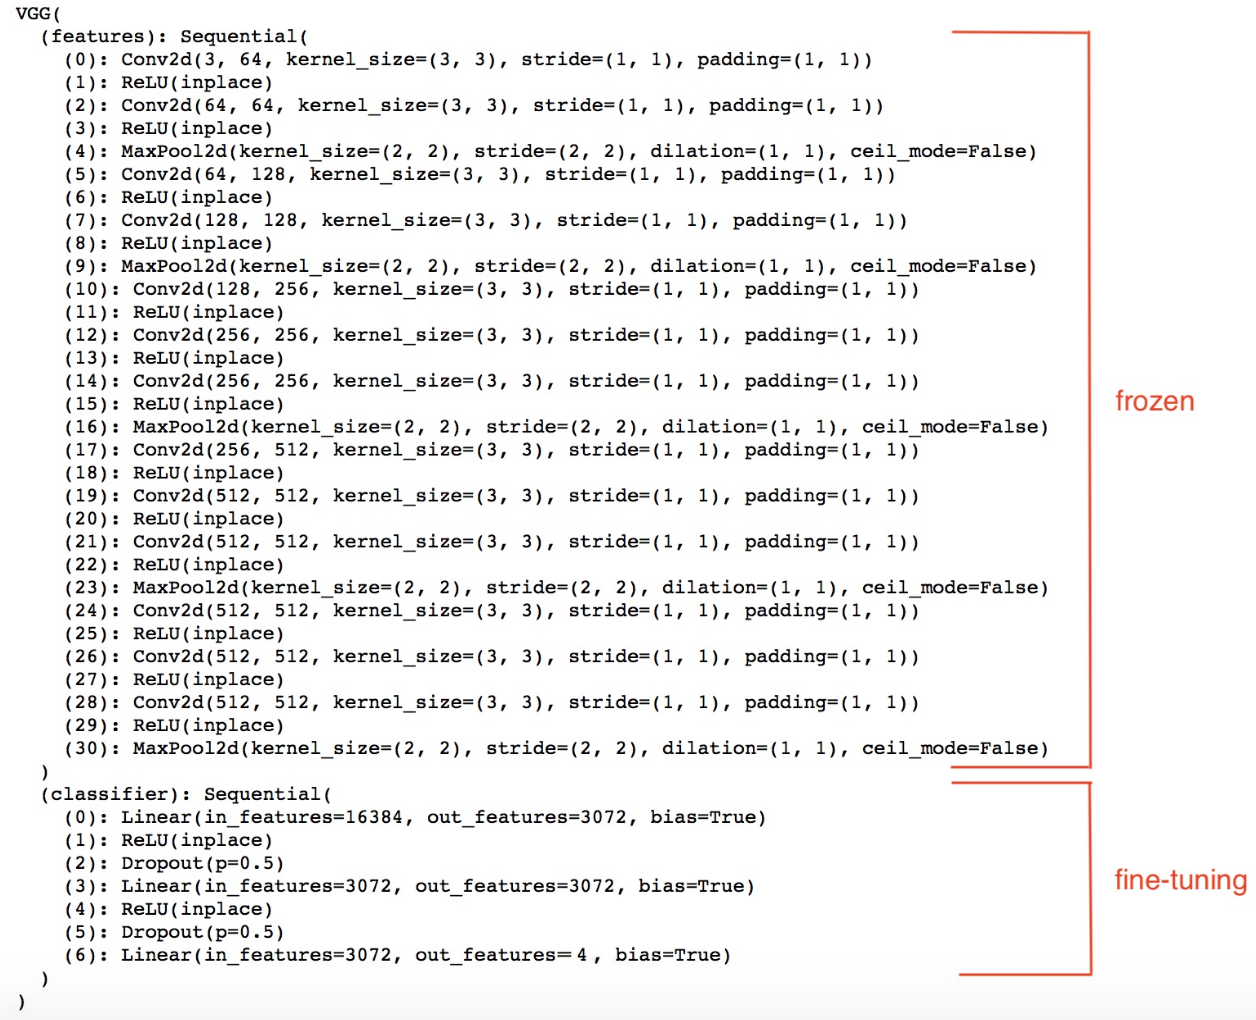
\includegraphics[scale=0.70]{image20.png}
\end{figure}
Poiché il task di regressione richiede in output 4 numeri reali x, y, u, v, sono stati modificati gli ultimi livelli lineari impostando a 4 le features di output dell’ultimo livello.
Per la procedura di training utilizziamo: 
\begin{itemize}
	\item[•]Learning rate: 0.00001
	\item[•]Momentum: 0.9
	\item[•]Weight decay: 0.000001
\end{itemize}
Come loss function da ottimizzare utilizziamo MSE loss, come funzione di attivazione utilizziamo ReLU, mentre come metodo di learning utilizziamo SGD. \\
Poiché abbiamo da stimare quattro numeri reali x, y, u, v, utilizziamo a tale scopo quattro loss functions, una per ogni valore, le quali verranno ottimizzate assieme durante la procedura di training. \\
Abbiamo allenato il modello per 400 epoche, ed abbiamo ottenuto i seguenti risultati:

\subsubsection{Loss functions}
\begin{figure}[H]
	\centering
	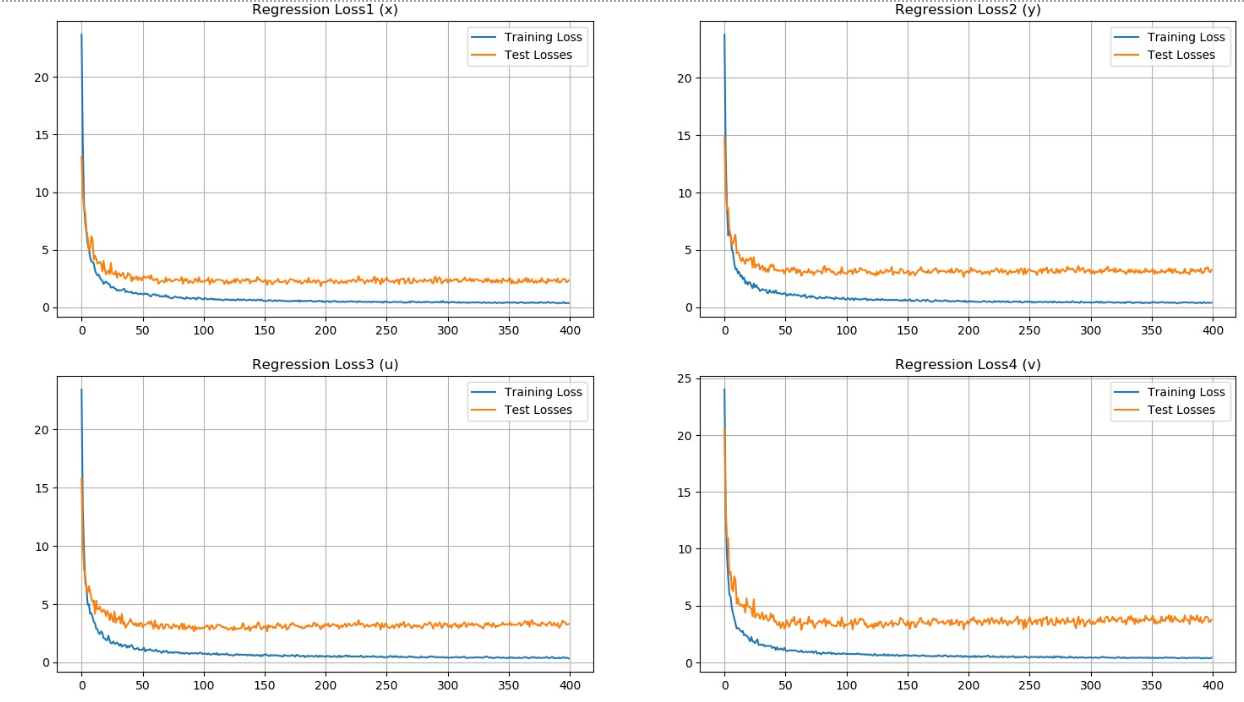
\includegraphics[scale=0.70]{image21.png}
\end{figure}
Come è possibile osservare le loss sul validation si avvicinano a quelle del training. Tuttavia ancora siamo lontani dai risultati ottimali avuti col metodo proposto.

\subsubsection{MSE errors}
\begin{center}
	\begin{tabular}{| l | l | l | l |}
		\hline
		MSE sul parametro X & 9.94 \\ \hline
		MSE sul parametro Y & 1.71 \\ \hline
		MSE sul parametro U & 0.10 \\ \hline
		MSE sul parametro V & 0.07 \\ \hline							
	\end{tabular}
\end{center}

\subsubsection{REC curves}
\begin{figure}[H]
	\centering
	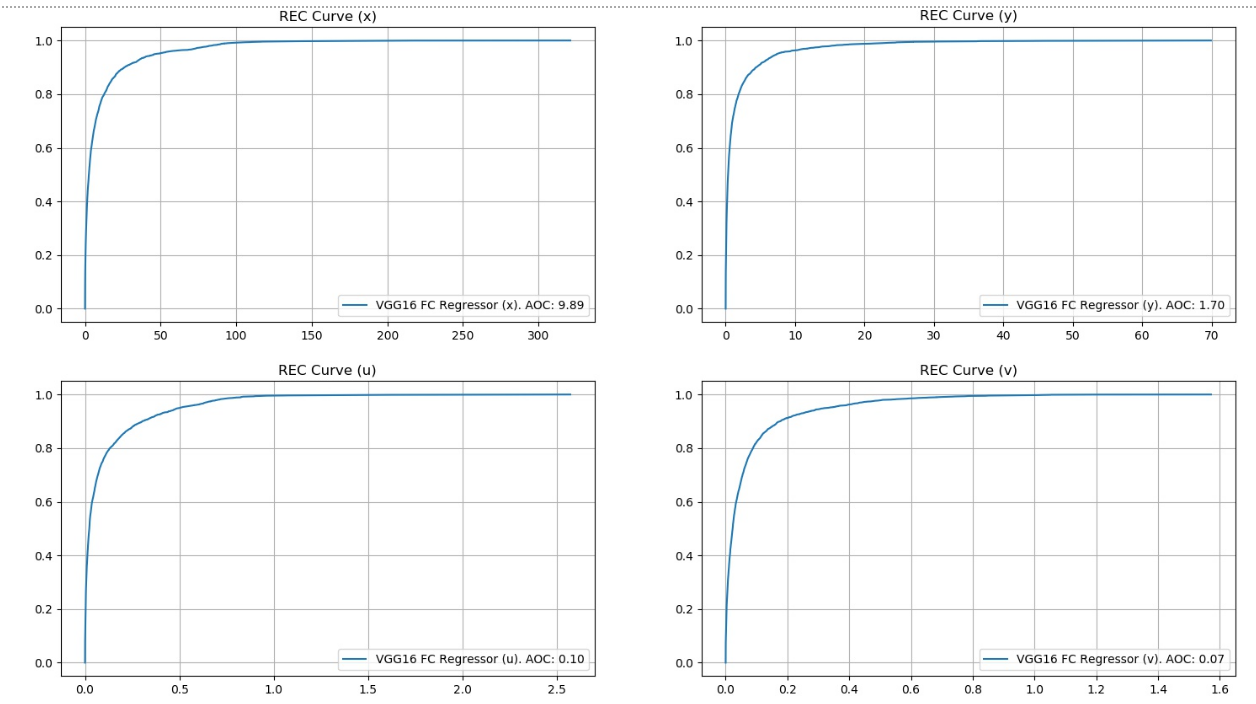
\includegraphics[scale=0.70]{image22.png}
\end{figure}

\subsubsection{RMS error}
errore RMS (Root Mean Square) medio e mediano relativo a posizione (in metri) e orientamento (in gradi):
\begin{center}
	\begin{tabular}{| l | l | l | l |}
		\hline
		Mean location error & 2.5976 \\ \hline
		Median location error & 1.9156 \\ \hline
		Mean orientation error & 12.9392 \\ \hline
		Median orientation error & 7.6587 \\ \hline							
	\end{tabular}
\end{center}

%==========================================
\section{VGG16 pre-addestrata: {2\textdegree} approccio}
Sono stati freezati tutti i livelli del modulo “features” che contiene i blocchi convoluzionali, ad eccezione dell’ultimo blocco. In questo modo verranno aggiornati solamente i parametri dei livelli del modulo “classifier”, ed i parametri dei livelli dell’ultimo blocco convoluzionale.
\subsection{Classificazione}
\begin{figure}[H]
	\centering
	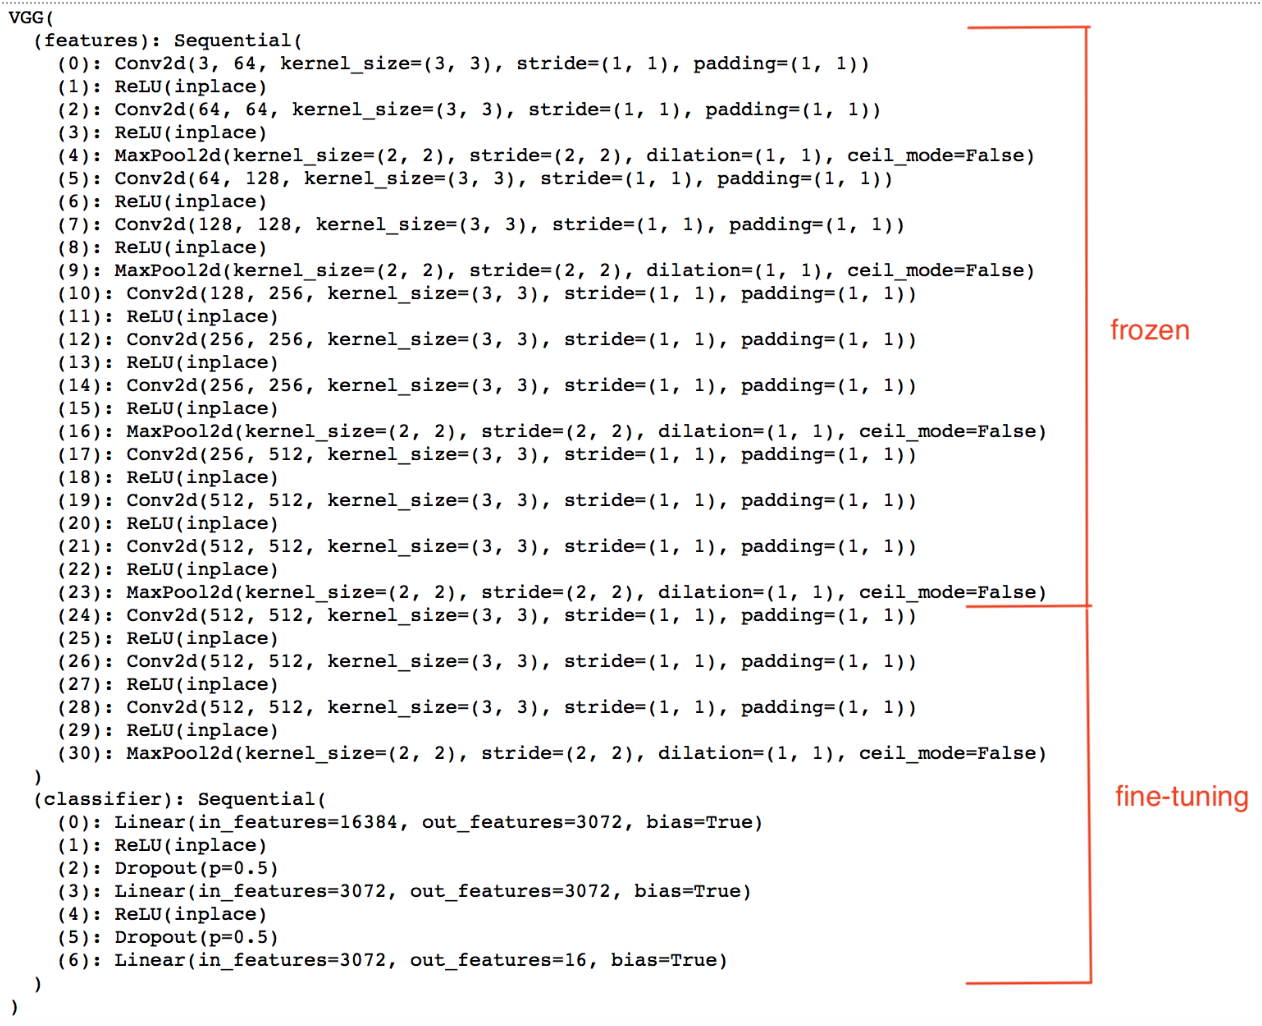
\includegraphics[scale=0.70]{image23.png}
\end{figure}
Poichè il task di classificazione richiede in output 16 classi, sono stati modificati gli ultimi livelli lineari impostando a 16 le features di output dell’ultimo livello con classificatore softmax.
Per la procedura di training utilizziamo: 
\begin{itemize}
	\item[•]Learning rate: 0.00001
	\item[•]Momentum: 0.9
	\item[•]Weight decay: 0.000001
\end{itemize}
Come loss function utilizziamo cross entropy loss, come funzione di attivazione utilizziamo ReLU, mentre come metodo di learning utilizziamo SGD. \\
Abbiamo allenato il modello per 400 epoche, ed abbiamo ottenuto i seguenti risultati:

\subsubsection{Accuracy}
\begin{figure}[H]
	\centering
	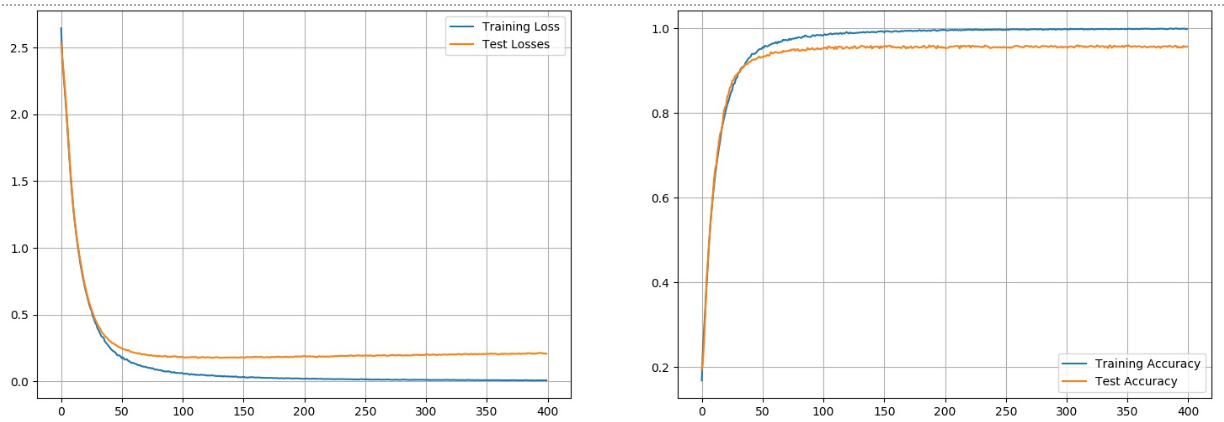
\includegraphics[scale=0.65]{image24.png}
\end{figure}
Dai plot, di cui sopra, è possibile osservare che i ottiene una accuracy relativamente alta: 0.96.

\subsubsection{Matrice di confusione}
\begin{figure}[H]
	\centering
	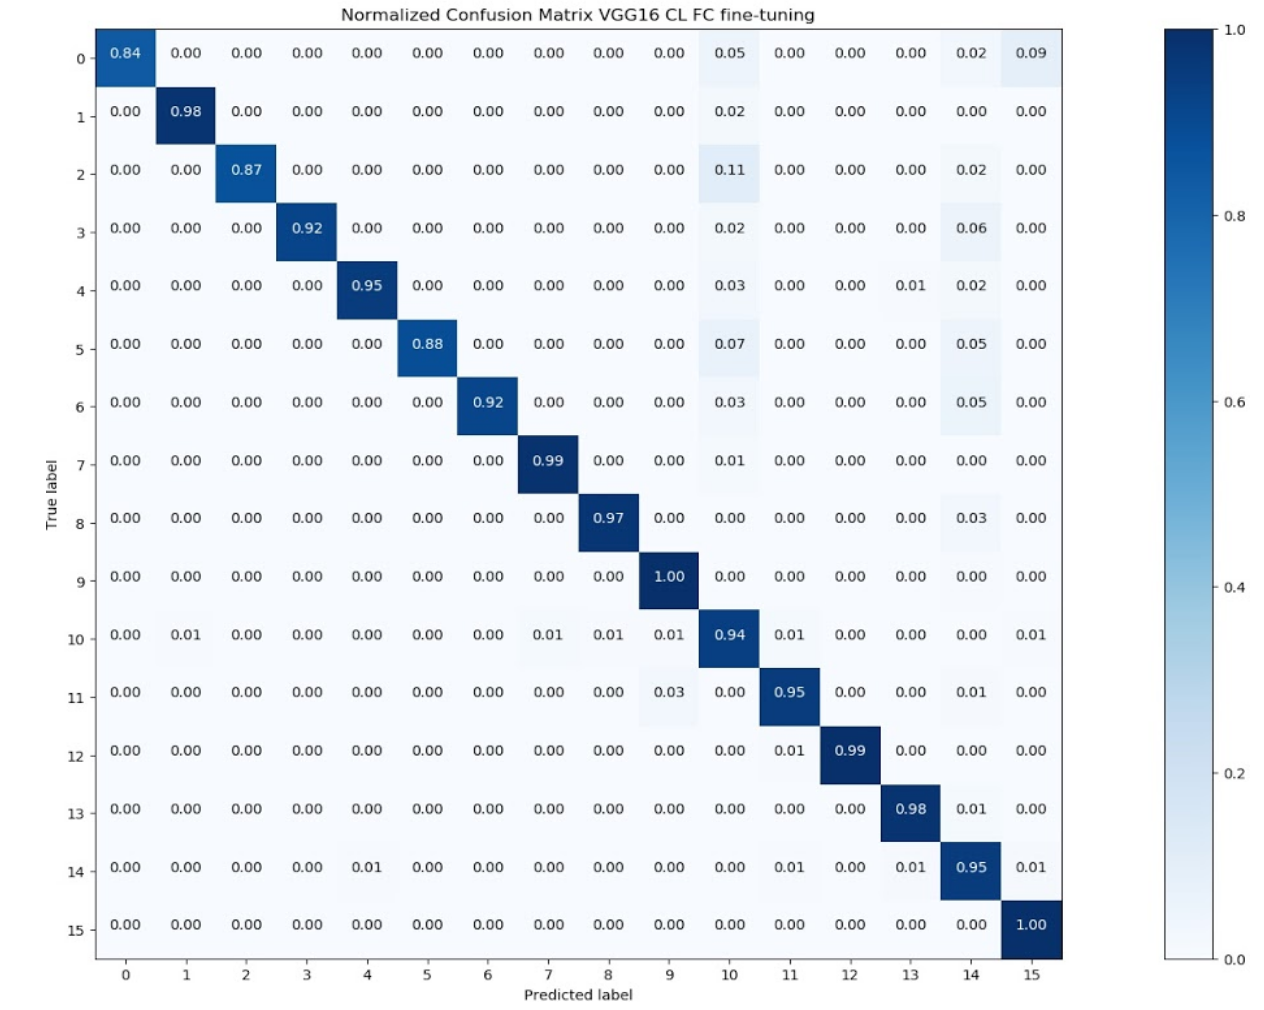
\includegraphics[scale=0.5]{image25.png}
\end{figure}
Abbiamo ottimi risultati sulla diagonale principale, infatti avremo degli score F1 maggiori.

\subsubsection{Score F1 e Score mF1}
\begin{center}
	\begin{tabular}{| l | l | l | l |}
		\hline
		Classe & Score F1 \\ \hline
		0 & 0.91 \\ \hline
		1 & 0.97 \\ \hline
		2 & 0.93 \\ \hline
		3 & 0.95 \\ \hline
		4 & 0.96 \\ \hline
		5 & 0.93 \\ \hline
		6 & 0.96 \\ \hline
		7 & 0.96 \\ \hline
		8 & 0.96 \\ \hline
		9 & 0.99 \\ \hline
		10 & 0.92 \\ \hline
		11 & 0.96 \\ \hline
		12 & 0.99 \\ \hline
		13 & 0.98 \\ \hline
		14 & 0.95\\ \hline
		15 & 0.96 \\ \hline 
		{\bf Score mF1} & 0.95 \\ \hline							
	\end{tabular}
\end{center}
Con questa architettura abbiamo raggiunto una {\bf accuracy} di {\bf 0.96} sul validation.

\subsection{Regressione}
\begin{figure}[H]
	\centering
	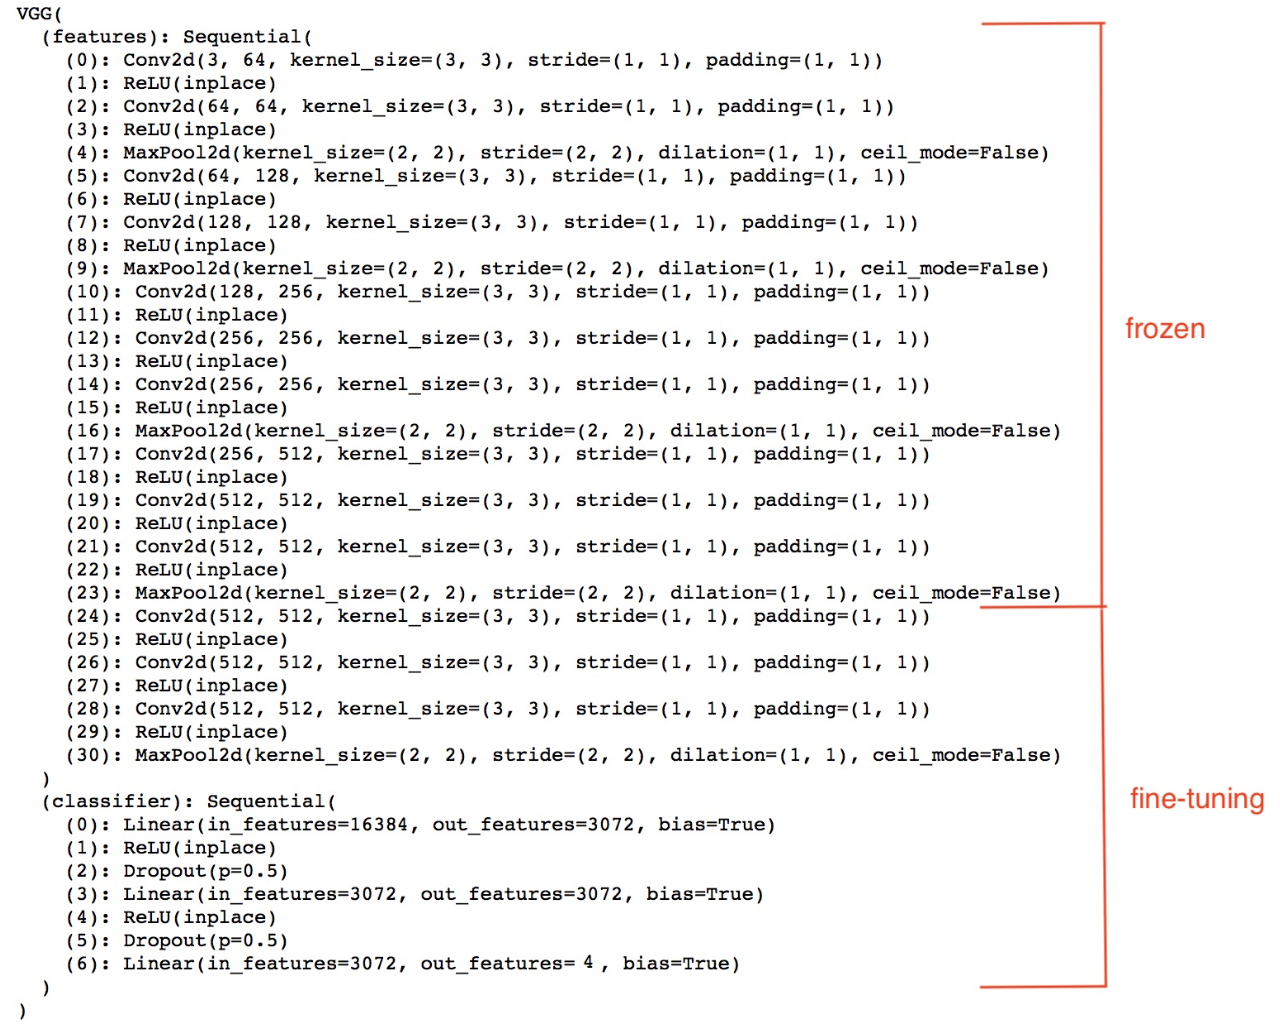
\includegraphics[scale=0.70]{image26.png}
\end{figure}
Poiché il task di regressione richiede in output 4 numeri reali x, y, u, v, sono stati modificati gli ultimi livelli lineari impostando a 4 le features di output dell’ultimo livello. \\
Per la procedura di training utilizziamo:
\begin{itemize}
	\item[•]Learning rate: 0.00001
	\item[•]Momentum: 0.9
	\item[•]Weight decay: 0.000001
\end{itemize} 
Come loss function da ottimizzare utilizziamo MSE loss, come funzione di attivazione utilizziamo ReLU, mentre come metodo di learning utilizziamo SGD. \\
Poiché abbiamo da stimare quattro numeri reali x, y, u, v, utilizziamo a tale scopo quattro loss functions, una per ogni valore, le quali verranno ottimizzate assieme durante la procedura di training. \\
Abbiamo allenato il modello per 400 epoche, ed abbiamo ottenuto i seguenti risultati:

\subsubsection{Loss functions}
\begin{figure}[H]
	\centering
	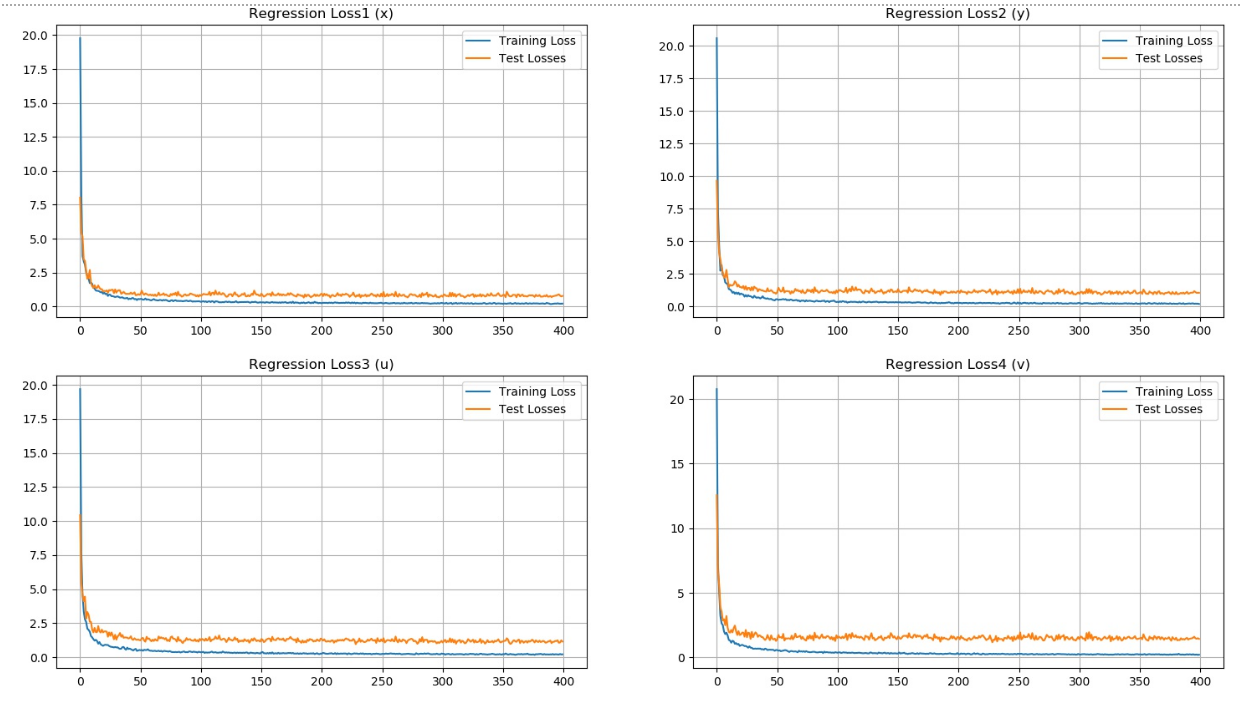
\includegraphics[scale=0.70]{image27.png}
\end{figure}

\subsubsection{MSE errors}
\begin{center}
	\begin{tabular}{| l | l | l | l |}
		\hline
		MSE sul parametro X & 3.55 \\ \hline
		MSE sul parametro Y & 0.85 \\ \hline
		MSE sul parametro U & 0.06 \\ \hline
		MSE sul parametro V & 0.04 \\ \hline							
	\end{tabular}
\end{center}

\subsubsection{REC curves}
\begin{figure}[H]
	\centering
	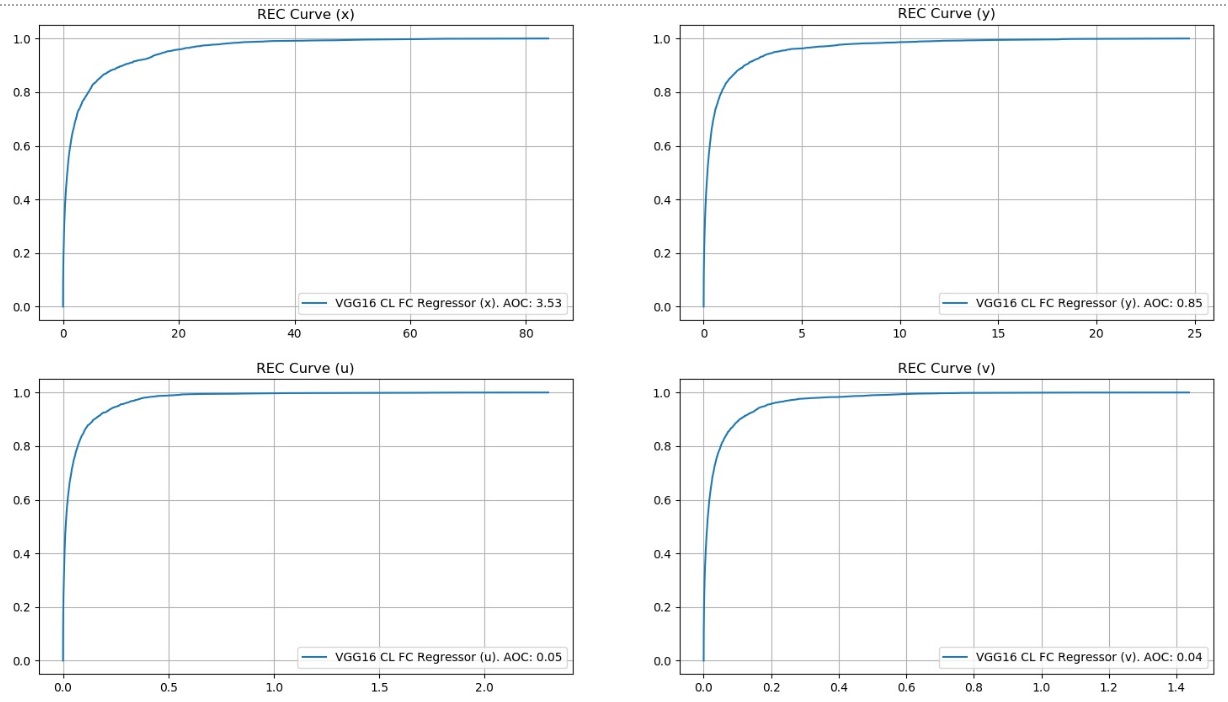
\includegraphics[scale=0.70]{image28.png}
\end{figure}

\subsubsection{RMS error}
errore RMS (Root Mean Square) medio e mediano relativo a posizione (in metri) e orientamento (in gradi):
\begin{center}
	\begin{tabular}{| l | l | l | l |}
		\hline
		Mean location error & 1.5754 \\ \hline
		Median location error & 1.1219 \\ \hline
		Mean orientation error & 8.7991 \\ \hline
		Median orientation error & 5.3730 \\ \hline							
	\end{tabular}
\end{center}

% [END]

%=====================

% [START] Capitolo 3
\chapter{Metodo Proposto}
Il metodo che ha fornito i migliori risultati, sia per il task di classificazione che per quello di regressione, è stato ottenuto affinando le diverse strategie sperimentate sopra elencate. Esso sfrutta ancora una volta l’architettura di rete VGG16 pre-addestrata sul dataset “ImageNet” e si basa essenzialmente sull’aggiunta di “data augmentation”, ovvero una tecnica che permette di aumentare i dati in maniera sintetica trasformando “al volo” i dati in input in maniera casuale e facendo in modo che, dopo la trasformazione, l’etichetta sia ancora valida, e su un opportuno “fine-tuning” della reta.\\
Ciò ci ha permesso di ottenere un modello più robusto e capace di generalizzare, riducendo l’overfitting.
Le trasformazioni, applicate solo in fase di training, sono le seguenti:
\begin{itemize}
	\item[•]Random Horizontal Flip: flip orizzontale random con probabilità 0.5
	\item[•]Color Jitter: il valore di ogni pixel viene perturbato leggermente in maniera casuale
	\item[•]Random Rotation(20): rotazione random dell’immagine tra -20° e +20°
	\item[•]Random Crop(128): crop 128x128 viene estratto casualmente dall’immagine
\end{itemize}
Per compatibilità, in fase di test vengono estratti crop 128x128 dalla parte centrale dell’immagine.
A seguito delle trasformazioni, siamo costretti ad adattare la struttura dell’architettura per accettare in input immagini da 128x128, andando essenzialmente a modificare i livelli lineari del blocco fully connected.
\\ \\
E’ stato effettuato poi il fine-tuning del modello, freezando tutti i livelli del modulo “features” che contiene i blocchi convoluzionali, ad eccezione degli ultimi due blocchi, e del blocco fully connected del modulo “classifier”. \\
In questo modo verranno aggiornati solamente i parametri dei livelli del blocco fully connected, ed i parametri dei livelli degli ultimi due blocchi convoluzionali. \\
Sono stati poi cambiati i dropout nei livelli fully connected, impostando come probabilità 0.25.

\section{Classificazione}
\begin{figure}[H]
	\centering
	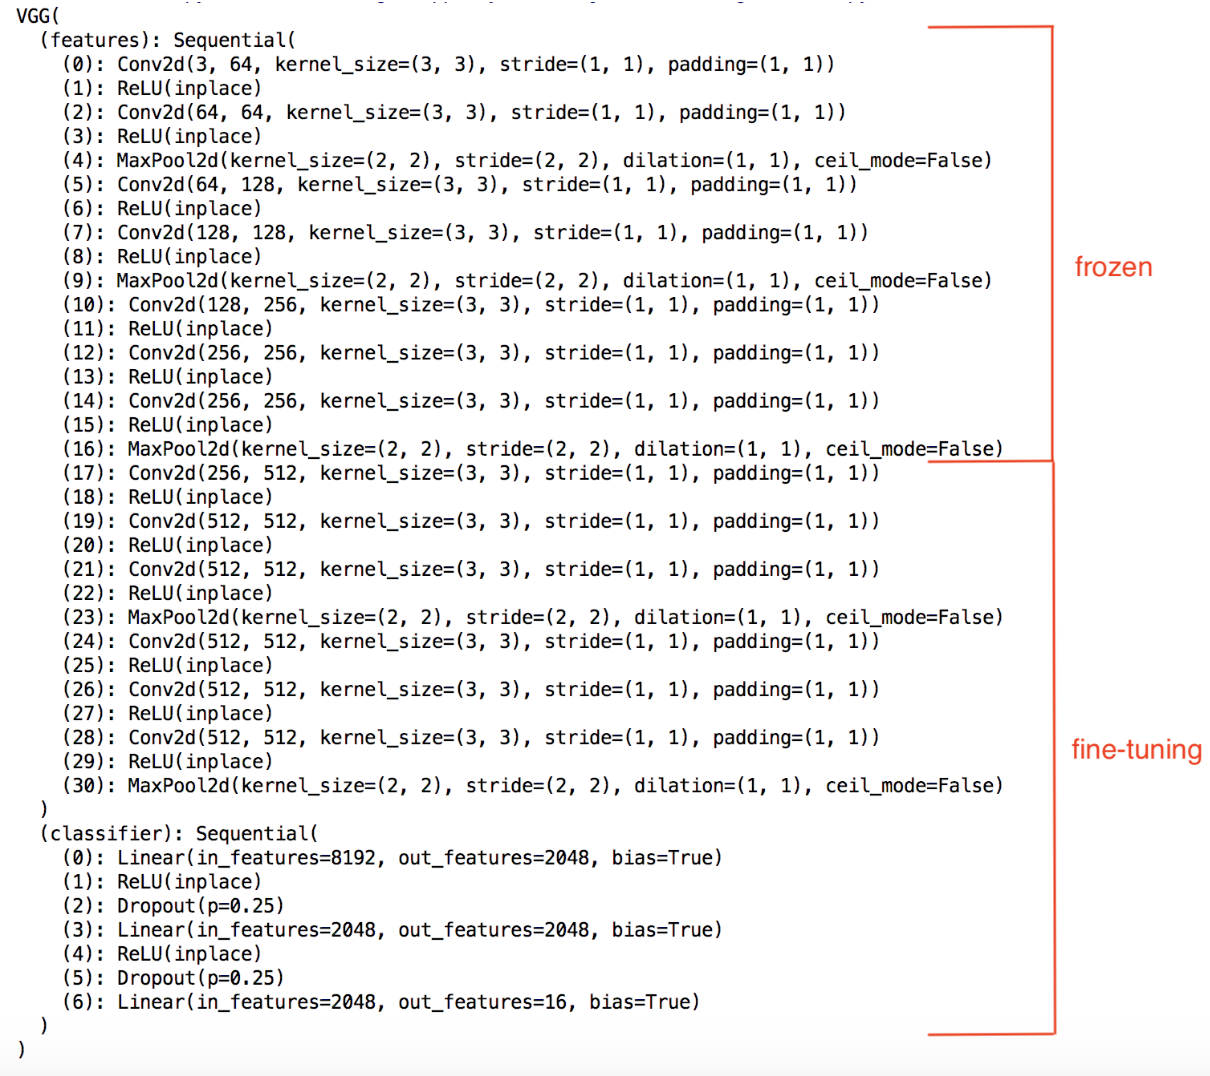
\includegraphics[scale=0.70]{image29.png}
\end{figure}
Poichè il task di classificazione richiede in output 16 classi, sono stati modificati gli ultimi livelli lineari impostando a 16 le features di output dell’ultimo livello con classificatore softmax.
Per la procedura di training utilizziamo: 
\begin{itemize}
	\item[•]Learning rate: 0.00001
	\item[•]Momentum: 0.9
	\item[•]Weight decay: 0.000001
\end{itemize}
Come loss function utilizziamo cross entropy loss, come funzione di attivazione utilizziamo ReLU, mentre come metodo di learning utilizziamo SGD. \\
Abbiamo allenato il modello per 400 epoche, ed abbiamo ottenuto i seguenti risultati:

\subsection{Accuracy}
\begin{figure}[H]
	\centering
	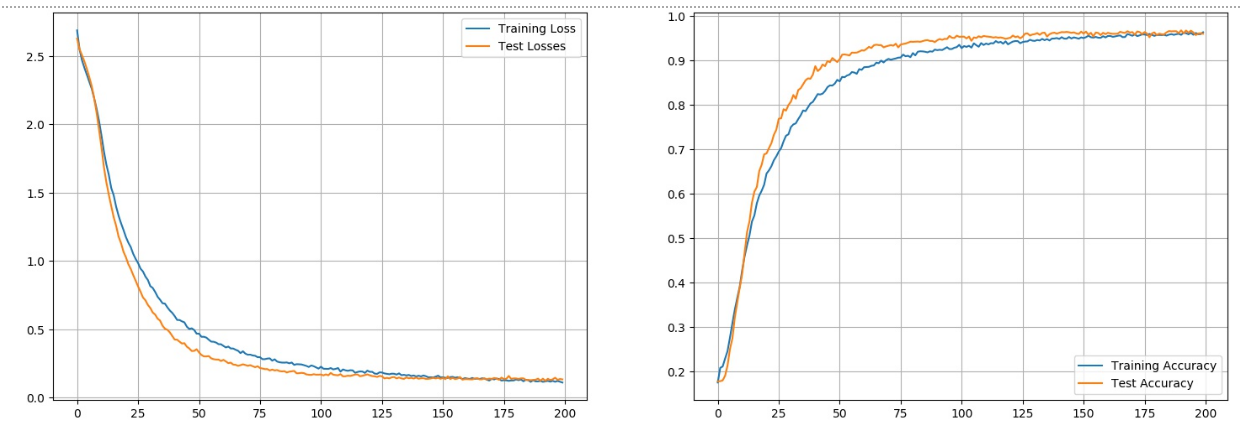
\includegraphics[scale=0.65]{image30.png}
\end{figure}
Dai due plot, di cui sopra, possiamo osservare la convergenza della validation/training loss e della validation/training accuracy.

\subsection{Matrice di confusione}
\begin{figure}[H]
	\centering
	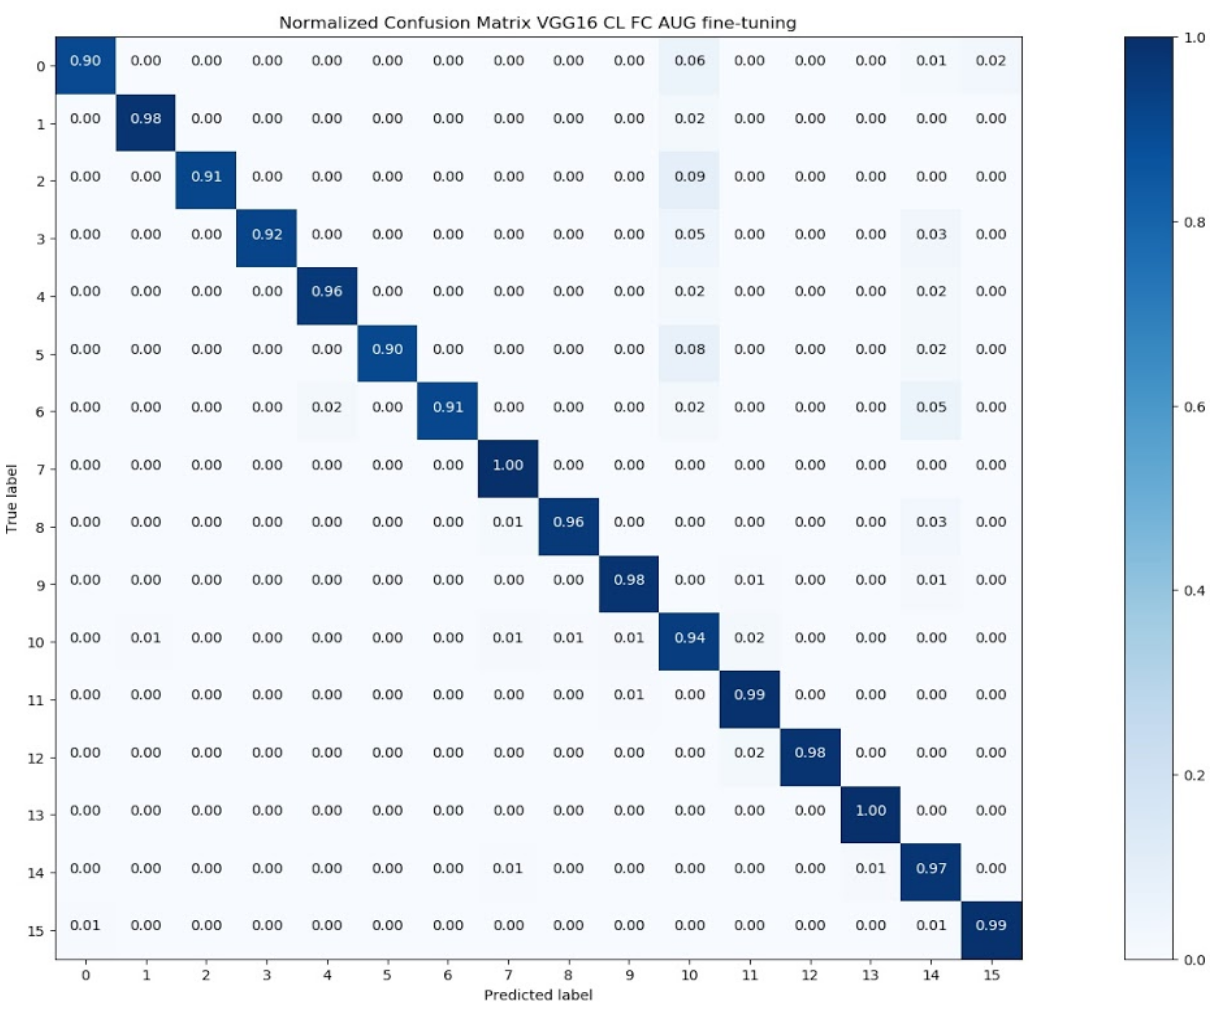
\includegraphics[scale=0.5]{image31.png}
\end{figure}

\subsection{Score F1 e Score mF1}
\begin{center}
	\begin{tabular}{| l | l | l | l |}
		\hline
		Classe & Score F1 \\ \hline
		0 & 0.94 \\ \hline
		1 & 0.97 \\ \hline
		2 & 0.95 \\ \hline
		3 & 0.95 \\ \hline
		4 & 0.97 \\ \hline
		5 & 0.94 \\ \hline
		6 & 0.95 \\ \hline
		7 & 0.95 \\ \hline
		8 & 0.96 \\ \hline
		9 & 0.98 \\ \hline
		10 & 0.92 \\ \hline
		11 & 0.97 \\ \hline
		12 & 0.99 \\ \hline
		13 & 0.99 \\ \hline
		14 & 0.97 \\ \hline
		15 & 0.99 \\ \hline 
		{\bf Score mF1} & 0.96 \\ \hline							
	\end{tabular}
\end{center}
Con questa architettura abbiamo raggiunto una {\bf accuracy} di {\bf 0.97} sul validation.

\section{Regressione}
\begin{figure}[H]
	\centering
	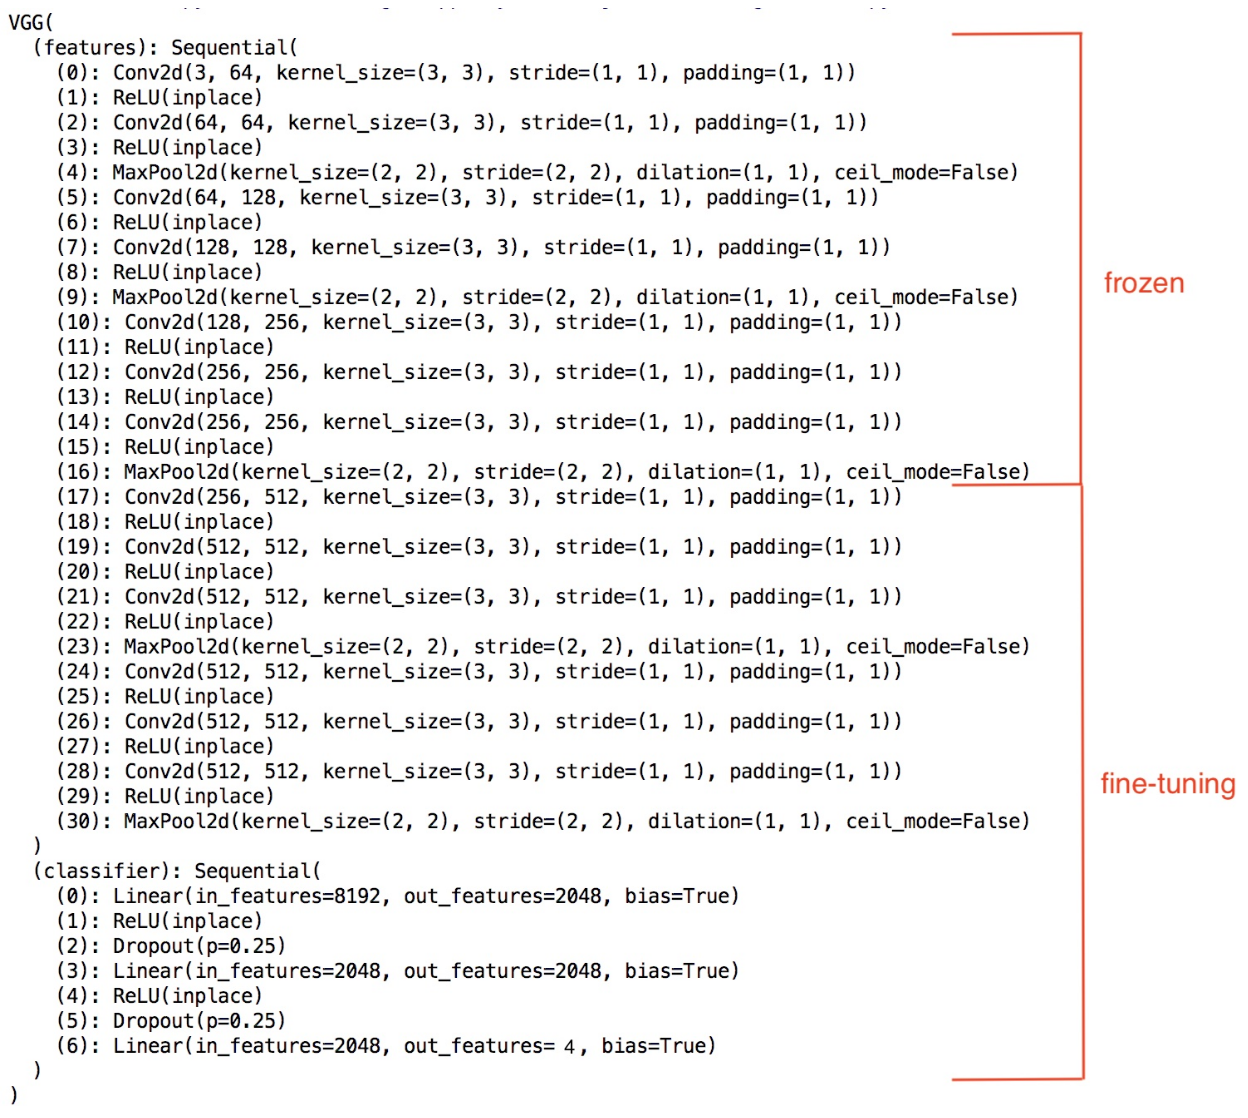
\includegraphics[scale=0.70]{image32.png}
\end{figure}
Poiché il task di regressione richiede in output 4 numeri reali x, y, u, v, sono stati modificati gli ultimi livelli lineari impostando a 4 le features di output dell’ultimo livello. \\
Per la procedura di training utilizziamo: 
\begin{itemize}
	\item[•]Learning rate: 0.00001
	\item[•]Momentum: 0.9
	\item[•]Weight decay: 0.000001
\end{itemize}
Come loss function da ottimizzare utilizziamo MSE loss, come funzione di attivazione utilizziamo ReLU, mentre come metodo di learning utilizziamo SGD. \\
Poiché abbiamo da stimare quattro numeri reali x, y, u, v, utilizziamo a tale scopo quattro loss functions, una per ogni valore, le quali verranno ottimizzate assieme durante la procedura di training. \\
Abbiamo allenato il modello per 400 epoche, ed abbiamo ottenuto i seguenti risultati:

\subsection{Loss functions}
\begin{figure}[H]
	\centering
	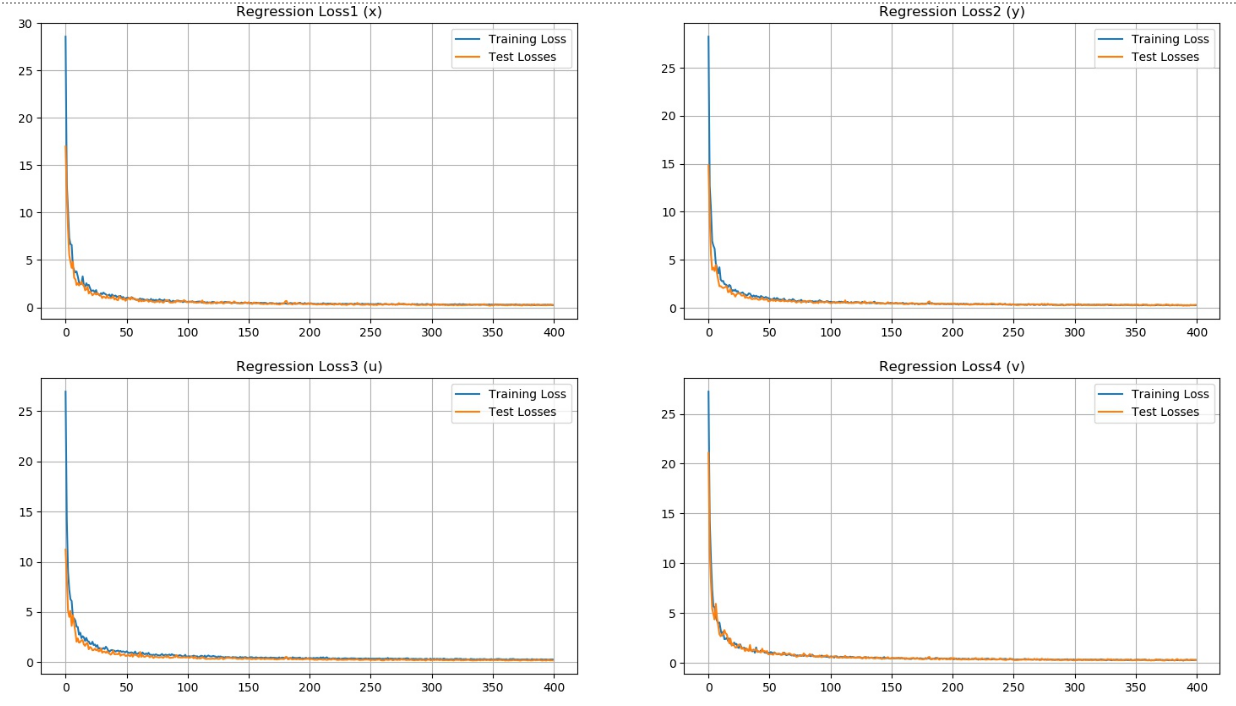
\includegraphics[scale=0.70]{image33.png}
\end{figure}
Dai 4 plot che mostrano le loss function, si può osservare come esse tendono a convergenza. A prova di ciò otteniamo valori ottimali con questa strategia.

\subsection{MSE errors}
\begin{center}
	\begin{tabular}{| l | l | l | l |}
		\hline
		MSE sul parametro X & 0.71 \\ \hline
		MSE sul parametro Y & 0.26 \\ \hline
		MSE sul parametro U & 0.05 \\ \hline
		MSE sul parametro V & 0.04 \\ \hline							
	\end{tabular}
\end{center}

\subsection{REC curves}
Le REC curve rappresentano un metodo grafico per valutare la bontà di un metodo di regressione. Inoltre, alla curva è spesso associata l'area sopra la curva (AOC) per offrire una misura dell'errore del metodo.
\begin{figure}[H]
	\centering
	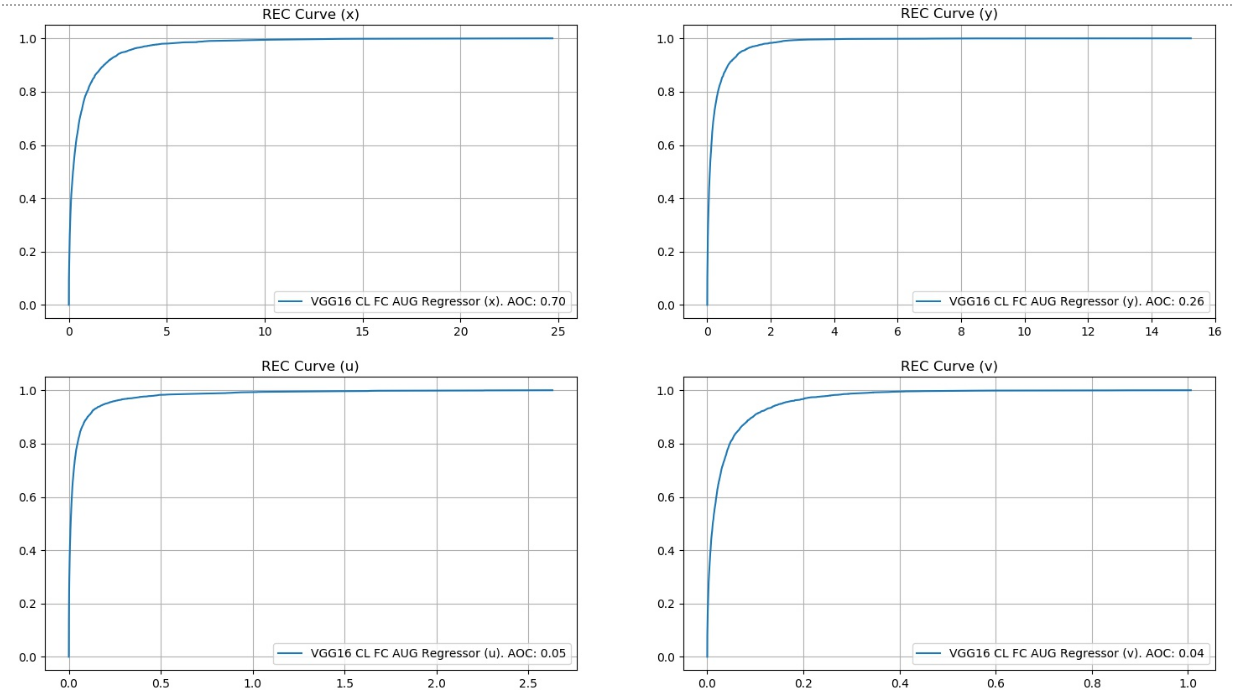
\includegraphics[scale=0.70]{image34.png}
\end{figure}

\subsubsection{RMS error}
errore RMS (Root Mean Square) medio e mediano relativo a posizione (in metri) e orientamento (in gradi):
\begin{center}
	\begin{tabular}{| l | l | l | l |}
		\hline
		Mean location error & 0.79 m \\ \hline
		Median location error & 0.65 m \\ \hline
		Mean orientation error & {9.60\textdegree} \\ \hline
		Median orientation error & {6.16\textdegree} \\ \hline							
	\end{tabular}
\end{center}
% [END]

%=====================

% [START] Conclusione
\chapter{Conclusioni}
In conclusione, ripercorriamo brevemente gli esperimenti condotti che ci hanno permesso di affrontare, nel migliore dei modi, i problemi di localizzazione basati su classificazione e regressione.
\\ \\
Abbiamo iniziato esplorando la neural network più conosciuta, la MLP, ed abbiamo utilizzato questa architettura su entrambi i task. \\
Dapprima una semplice MLP con un solo livello nascosto, poi con una MLP più profonda con due livelli nascosti. Con entrambe le architetture non abbiamo però ottenuto dei risultati soddisfacenti, ma addirittura ci siamo accorti di una peculiarità: rendendo più complessa l’architettura, aggiungendo più livelli, le performance del modello peggioravano. Questo comportamento indica come l’architettura MLP non riesce a trovare i parametri corretti e non si adatta bene a lavorare su problemi che hanno a che fare con le immagini.
\\ \\
Per questo motivo, ci siamo orientati sulle CNN, le quali permettono di applicare le reti neurali in maniera efficiente al processamento di immagini. Esse sostituiscono le trasformazioni lineari con le convoluzioni, che richiedono meno parametri e permettono di conservare le informazioni spaziali. \\
Come primo passo abbiamo ripreso l’architettura di rete VGG16 pre-addestrata su “ImageNet” ed eseguito tre diversi approcci di fine-tuning sulla rete: con i primi due abbiamo di volta in volta aumentato i blocchi, e quindi il numero di parametri, coinvolti nell’aggiornamento, mantenendo le low level features di VGG16, mentre con l’ultimo approccio abbiamo inoltre optato per l’aggiunta di data augmentation ed una serie di trasformazioni per provare a generalizzare meglio il modello.
\\ \\
Ci siamo accorti come i risultati dei primi due approcci sono simili tra loro, ma che, all’aumentare dei livelli “sfreezati”, occorreva meno tempo a raggiungere la convergenza. \\
L’ultimo approccio invece è risultato essere il migliore, in quanto, con “sfreeze” degli ultimi due blocchi convoluzionali e del blocco fully connected finale insieme alla data augmentation, ci hanno permesso di ottenere i seguenti risultati:
\begin{itemize}
	\item[•]In classificazione: {\bf validation accuracy = 0.97 }
	\item[•]In regressione:
\end{itemize}
\begin{center}
	\begin{tabular}{| l | l | l | l |}
		\hline
		Mean Location Error & 0.79 m \\ \hline
		Median Location Error & 0.65 m \\ \hline
		Mean Orientation Error & {9.60\textdegree} \\ \hline
		Median Orientation Error & {6.16\textdegree} \\ \hline							
	\end{tabular}
\end{center}
In conclusione, possiamo ritenerci soddisfatti dei risultati ottenuti per quanto riguarda il task di classificazione. Avremmo potuto effettuare altri esperimenti, provando magari ad impostare un learning rate adattivo che si riducesse all’aumentare del numero delle epoche secondo determinate condizioni, o magari provare altre combinazioni di parametri per affinare i risultati oppure un’altra architettura studiata ad hoc, ma il costo computazionale e il conseguente impatto in termini temporali ci avrebbe impedito di rispettare i termini di scadenza per la consegna del progetto.\\
Per quanto riguarda invece il task di regressione, possiamo anche qui ritenerci abbastanza soddisfatti dei risultati ottenuti, anche se con un pò di rammarico nel non aver magari provato ad integrare, assieme alla CNN, una LSTM che avrebbe sfruttato le dipendenze e la natura sequenziale dei dati in input facilitando magari le performance dell’apprendimento e quindi la qualità dei risultati ottenuti.
% [END]

%=====================

% [START] Bibliografia
%\chapter*{Riferimenti bibliografici}
\addcontentsline{toc}{chapter}{Riferimenti bibliografici}
\markboth{Riferimenti bibliografici}{Riferimenti bibliografici}

\begin{itemize}

  \item[1.] Simone Faro, Thierry Lecroq: The exact online string matching problem: A review of the most recent results. ACM Comput. Surv. 45(2): 13 (2013)
  
  \item[2.] Domenico Cantone, Simone Faro, Emanuele Giaquinta: A compact representation of nondeterministic (suffix) automata for the bit-parallel approach. Inf. Comput. 213: 3-12 (2012)   
  
\end{itemize}
% [END]

%=====================


\end{document}